% !TeX root = ../main.tex

\chapter{相关技术基础}

本文工作开展在基于深度学习的神经辐射场之上,通过结合可微渲染实现了数字资产解耦管线,
致力于无缝对接传统渲染管线并解决其中的耦合问题。本章将介绍本文研究所必要的深度学习基础、
可微渲染理论基础、传统渲染管线介绍以及神经辐射场理论基础。

\section{深度学习基础}

深度学习是一种基于多层神经网络的机器学习方法,近年来备受关注并广泛应用。其核心在于利用深度神经网络解决复杂任务,
并已在多个领域产生深远影响。尤其在计算机视觉和图形学研究中,深度学习显著提升了任务性能,
逐步取代传统基于手工特征和规则的方法,成为当前研究的热点。本节将介绍深度学习的基础知识,包括网络基本模块与训练优化算法等内容。

\subsection{多层感知机}

多层感知机(Multilayer Perceptron,MLP)是深度学习的基础模型之一,由多个神经元层组成。
神经元的任务可以被划分为线性变换和非线性变换两部分。每个神经元能够接收多个输入值,
并根据自身的权重对输入值加权求和,随后应用激活函数以施加非线性变换。
单个神经元的结构如图~\ref{fig:neuron}所示。

\begin{figure}[htb]
  \centering
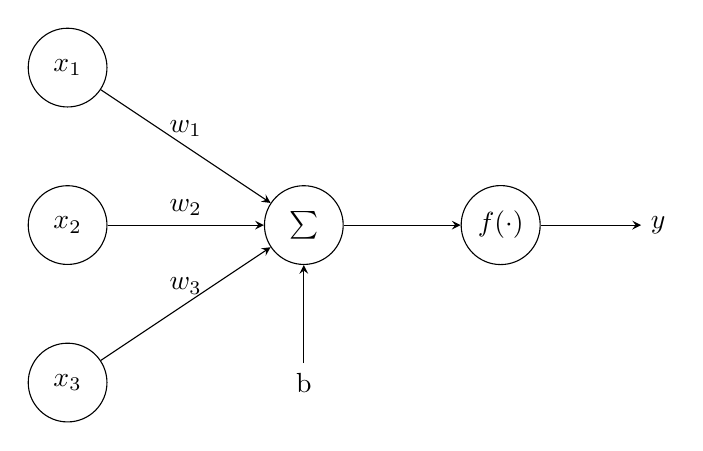
\begin{tikzpicture}[->,>=stealth, node distance=1.5cm, auto]
  % 定义输入节点
  \node[circle, draw, minimum size=1cm] (x1) at (0, 2) {$x_1$};
  \node[circle, draw, minimum size=1cm] (x2) at (0, 0) {$x_2$};
  \node[circle, draw, minimum size=1cm] (x3) at (0, -2) {$x_3$};

  % 定义偏置节点
  \node (bias) at (3, -2) {$\mathrm{b}$};

  % 定义神经元节点,内部写上激活函数(如 f(·))
  \node[circle, draw, minimum size=1cm] (sum) at (3, 0) {$\sum$};

  % 从输入节点到神经元的连线,并标注权重
  \draw (x1) -- node[midway, above] {$w_1$} (sum);
  \draw (x2) -- node[midway, above] {$w_2$} (sum);
  \draw (x3) -- node[midway, above] {$w_3$} (sum);
  % 从偏置节点到神经元的连线,标注偏置项
  \draw (bias) -- node[midway, below] {}(sum);

  % 定义神经元节点,内部写上激活函数(如 f(·))
  \node[circle, draw, minimum size=1cm] (activate) at (5.5, 0) {$f(\cdot)$};

  \node (y) at (7.5, 0) {$y$};

  \draw (sum) -- node[midway, below] {}(activate);
  \draw (activate) -- node[midway, below] {}(y);
\end{tikzpicture}
\caption{神经元的结构示意图}
\label{fig:neuron}
\end{figure}

通过神经元的层层传递,MLP逐步学习参数权重和偏置项,将输入映射到目标输出,实现分类、回归等任务。
MLP的结构如图~\ref{fig:mlp}所示。

\begin{figure}[htb]
  \centering
  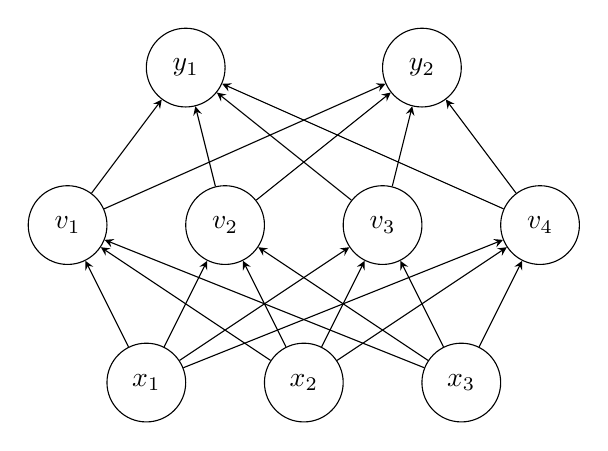
\begin{tikzpicture}[>=stealth, auto]

    % 定义公共变量
    \def\xspacing{2}      % 输入层和隐藏层的水平间距
    \def\layersep{2}       % 垂直层间距
    
    % 定义输出层特有的水平间距(可以调大该值)
    \def\outputxspacing{3} % 输出层水平间距
  
    % 输入层:3个节点
    \foreach \i in {1,...,3} {
      \pgfmathsetmacro{\xpos}{(\i-2)*\xspacing};
      \node[circle, draw, minimum size=1cm] (x\i) at (\xpos, 0) {$x_{\i}$};
    }
  
    % 隐藏层:4个节点
    \foreach \i in {1,...,4} {
      \pgfmathsetmacro{\xpos}{(\i-2.5)*\xspacing};
      \node[circle, draw, minimum size=1cm] (v\i) at (\xpos, \layersep) {$v_{\i}$};
    }
  
    % 输出层:2个节点,使用新的水平间距
    \foreach \i in {1,...,2} {
      \pgfmathsetmacro{\xpos}{(\i-1.5)*\outputxspacing};
      \node[circle, draw, minimum size=1cm] (y\i) at (\xpos, 2*\layersep) {$y_{\i}$};
    }
  
    % 连接输入层到隐藏层(全连接)
    \foreach \i in {1,...,3} {
      \foreach \j in {1,...,4} {
        \draw[->] (x\i) -- (v\j);
      }
    }
    
    % 连接隐藏层到输出层(全连接)
    \foreach \i in {1,...,4} {
      \foreach \j in {1,...,2} {
        \draw[->] (v\i) -- (y\j);
      }
    }
  
  \end{tikzpicture}
\caption{多层感知机的结构示意图}
\label{fig:mlp}
\end{figure}

根据通用近似定理\cite{Hornik_1989},只要网络拥有足够多的神经元,MLP就能拟合多种复杂的数据规律。
这一理论奠定了MLP作为函数逼近器的数学基础。然而,传统MLP需要将数据作为向量输入,通常缺乏明确的几何和空间结构信息,
因此难以处理三维空间建模等需要空间理解的任务。为了突破MLP在几何建模中的局限,
研究者提出了基于坐标的MLP(Coordinate-based MLPs),即直接将空间坐标作为网络输入。
但直接使用原始坐标输入MLP会导致明显的频谱偏差\cite{pmlr-v97-rahaman19a},
即网络倾向于优先学习低频信号,难以捕捉表面纹理或尖锐边缘等高频细节。为解决这一问题,
Tancik等人\cite{tancik2020fourier}引入了傅里叶坐标编码(Fourier Positional Encoding),
利用傅里叶基函数将$d$维坐标$\boldsymbol{x}\in\mathbb{R}^d$投影至高维空间。其计算方式如下:
\begin{equation}
\gamma(\boldsymbol{x})=\left[\sin\left(2^0\pi \boldsymbol{x}\right),\cos\left(2^\pi \boldsymbol{x}\right),\ldots,\sin\left(2^{K-1}\pi \boldsymbol{x}\right),\cos\left(2^{K-1}\pi \boldsymbol{x}\right)\right]
\label{eq:fourier_encoding}
\end{equation}
其中$K$表示频率层级。傅里叶坐标编码有效缓解了频谱偏差,使得MLP能够用于体积或者空间的建立,为后续的神经表示任务奠定了技术基础。

\subsection{激活函数}

MLP通过激活函数引入非线性变换,使网络具备更强的表示能力,因此,不同激活函数的特性将直接影响模型性能,
针对不同任务需选择合适的激活函数。常见的激活函数包括
Sigmoid、ReLU(Rectified Linear Unit)、ELU(Exponential Linear Unit)及Sinumoid。

\subsubsection*{(1)Sigmoid激活函数}

Sigmoid是一种平滑的S形函数,常用于早期的神经网络。Sigmoid函数的定义及导数计算如公式\eqref{eq:sigmoid}所示,
对应图像见图\ref{fig:sigmoid}。
\begin{equation}
  \begin{aligned}
  \text{Sigmoid}(x) &= \frac{1}{1+e^{-x}}, \\
  \text{Sigmoid}'(x) &= \text{Sigmoid}(x)\Bigl(1-\text{Sigmoid}(x)\Bigr).
  \end{aligned}
  \label{eq:sigmoid}
\end{equation}

Sigmoid函数的图像如图\ref{fig:sigmoid}所示,其输出范围在$(0,1)$之间,可以将任意实数映射到有限区间,
实现非线性变换。但是,当输入值较大或较小时,Sigmoid的导数会趋近于0,有可能会导致深层网络出现梯度爆炸的问题。
其次,由于Sigmoid的输出始终为正数,因此反向传播时所有权重的更新方向相同,进而降低训练过程的效率,影响收敛速度。
\begin{figure}[H]
  \centering
  \begin{subfigure}[t]{0.45\textwidth}
    \centering
    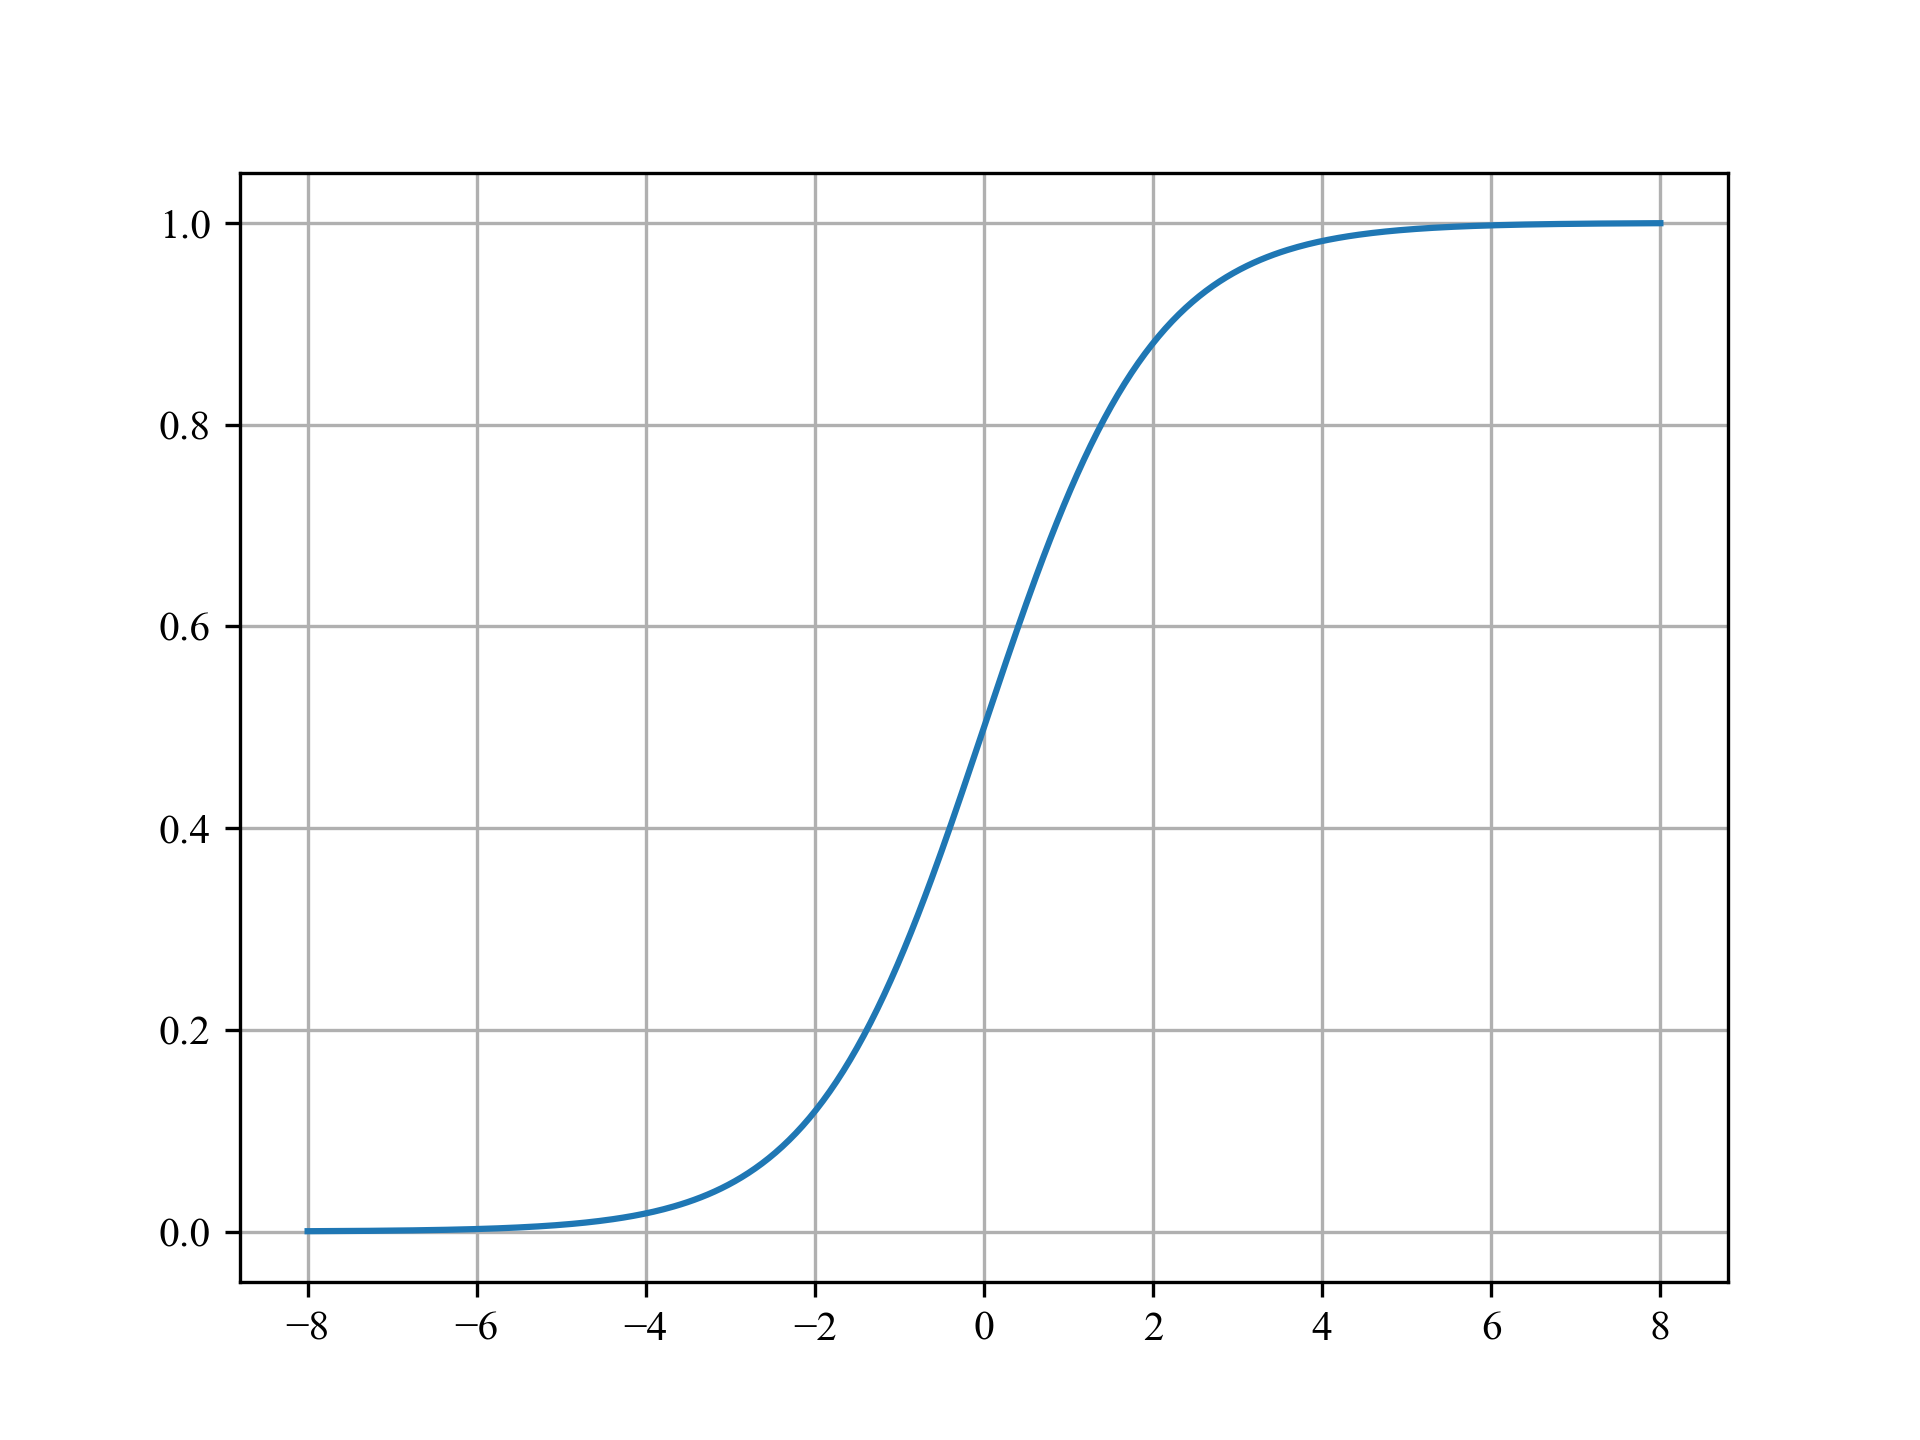
\includegraphics[width=\linewidth]{ch2/activation_function/sigmoid.png}
    \caption{Sigmoid函数图像}
  \end{subfigure}
  \begin{subfigure}[t]{0.45\textwidth}
    \centering
    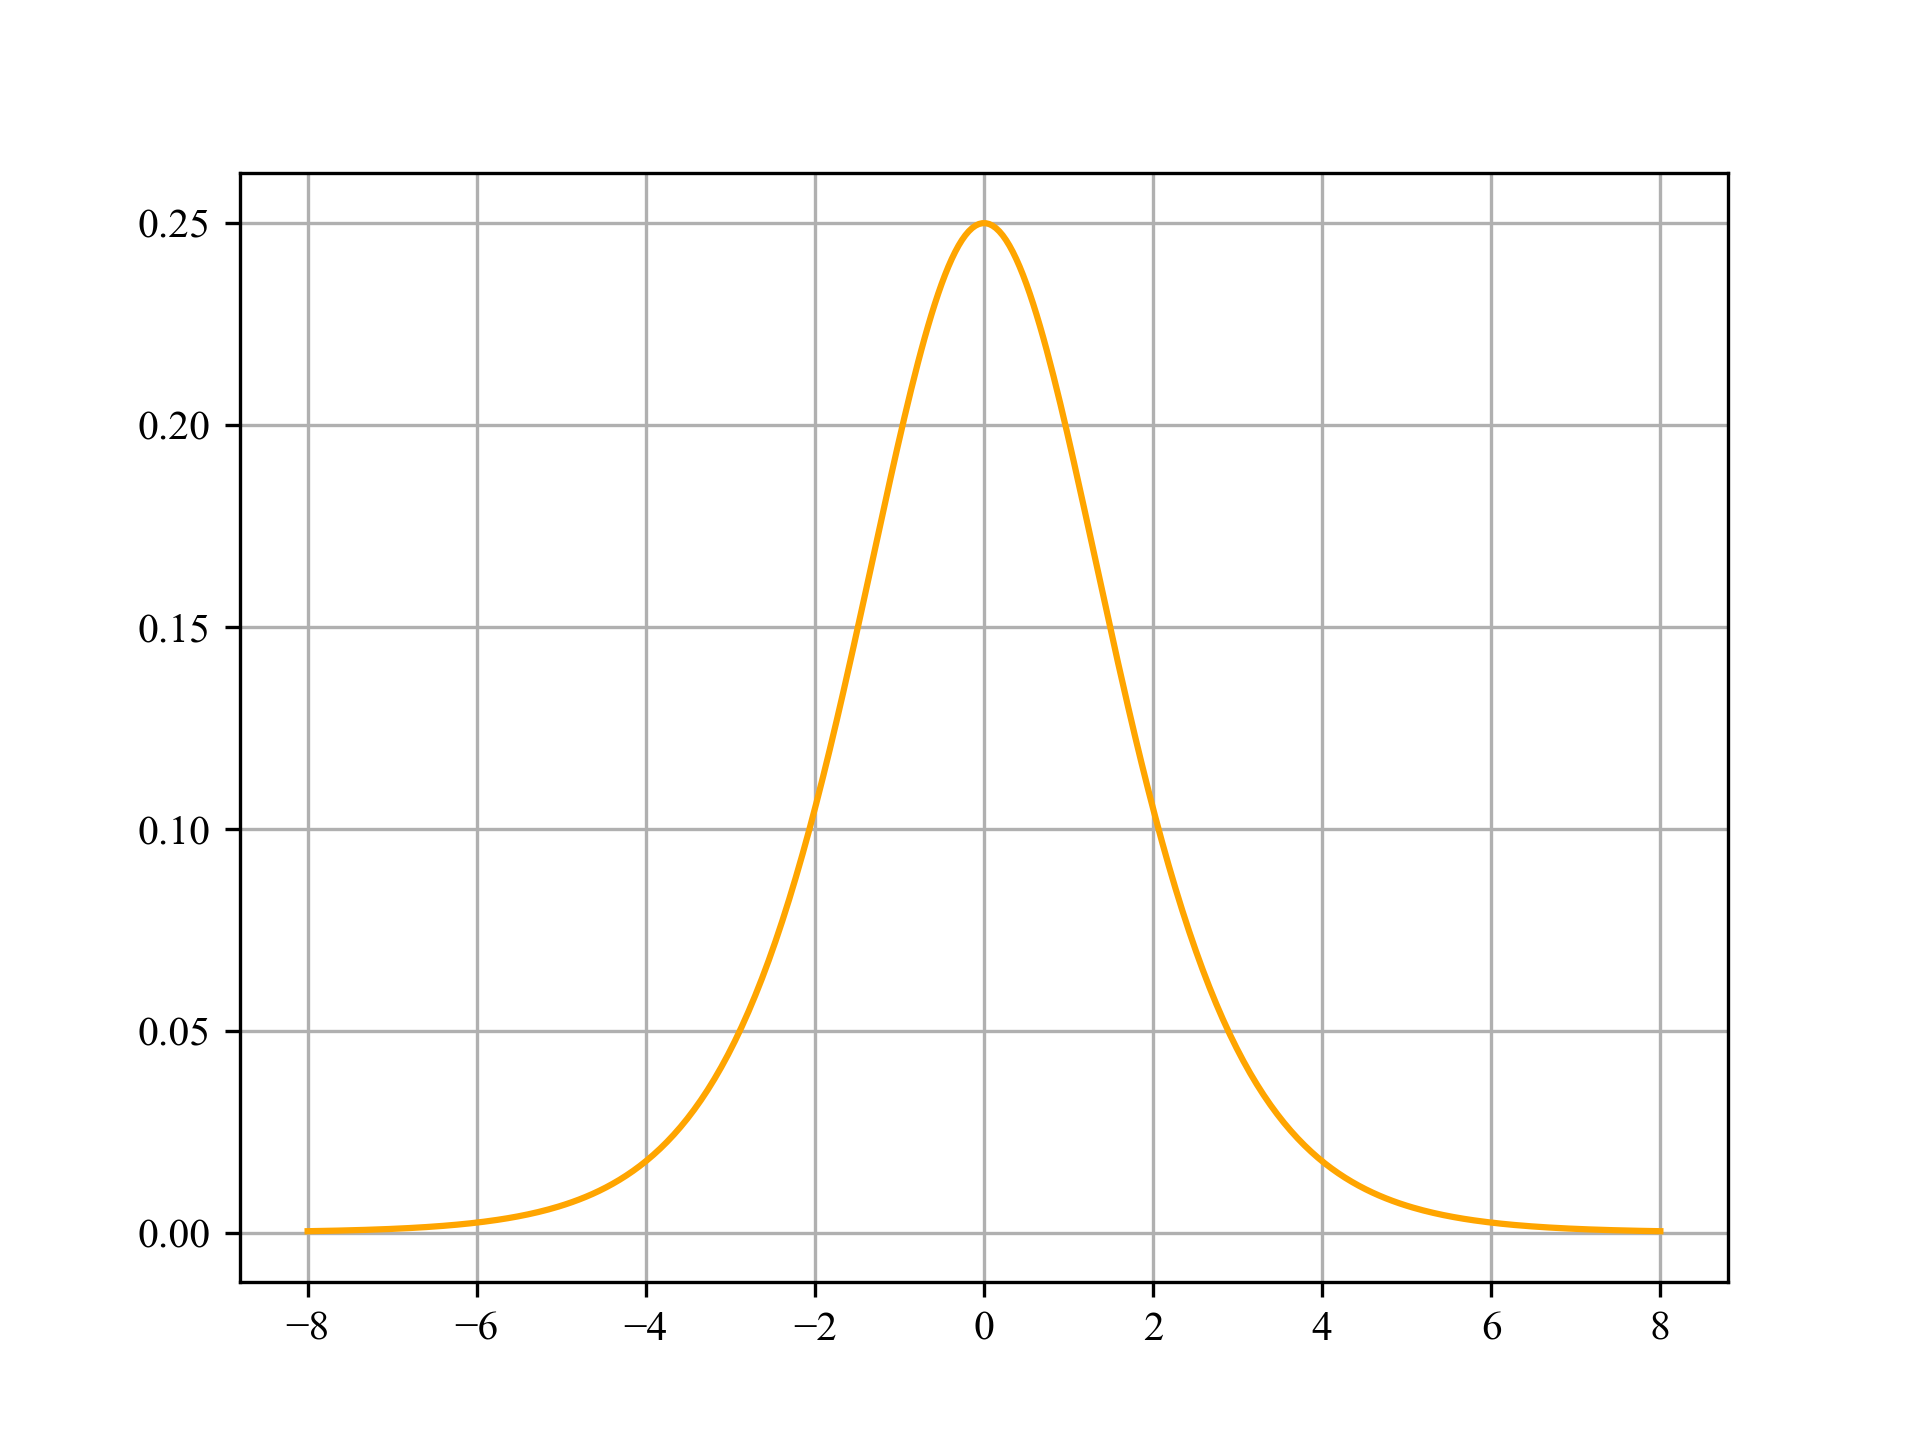
\includegraphics[width=\linewidth]{ch2/activation_function/dsigmoid.png}
    \caption{Sigmoid函数导数图像}
  \end{subfigure}
  \caption{Sigmoid激活函数及其导数图像}
  \label{fig:sigmoid}
\end{figure}

\subsubsection*{(2)ReLU激活函数}

ReLU激活函数由Nair等人\cite{Nair_Hinton_2010}提出,是一种分段函数,其基本表达式如公式\eqref{eq:relu}所示:
\begin{equation}
  \begin{aligned}
  \text{ReLU}(x) &= \begin{cases}
    0, & x < 0, \\
    x, & x \geq 0.
    \end{cases} \\
  \text{ReLU}'(x) &= \begin{cases}
  0, & x < 0, \\
  1, & x \geq 0.
  \end{cases}
  \end{aligned}
  \label{eq:relu}
\end{equation}

ReLU函数的图像如图\ref{fig:relu}所示,该函数近年来应用广泛。相较于Sigmoid函数,ReLU无需指数计算,因此计算效率更高。
同时,当输入大于0时,ReLU的导数始终为1,可以缓解Sigmoid激活函数梯度爆炸的问题;而当输入小于0时,ReLU输出恒为0,
这使得部分神经元不参与计算,能够增强网络的稀疏性,但此时ReLU导数也为0,因此可能会导致某些神经元“死亡”,影响网络的训练和收敛。
\begin{figure}[H]
  \centering
  \begin{subfigure}[t]{0.45\textwidth}
    \centering
    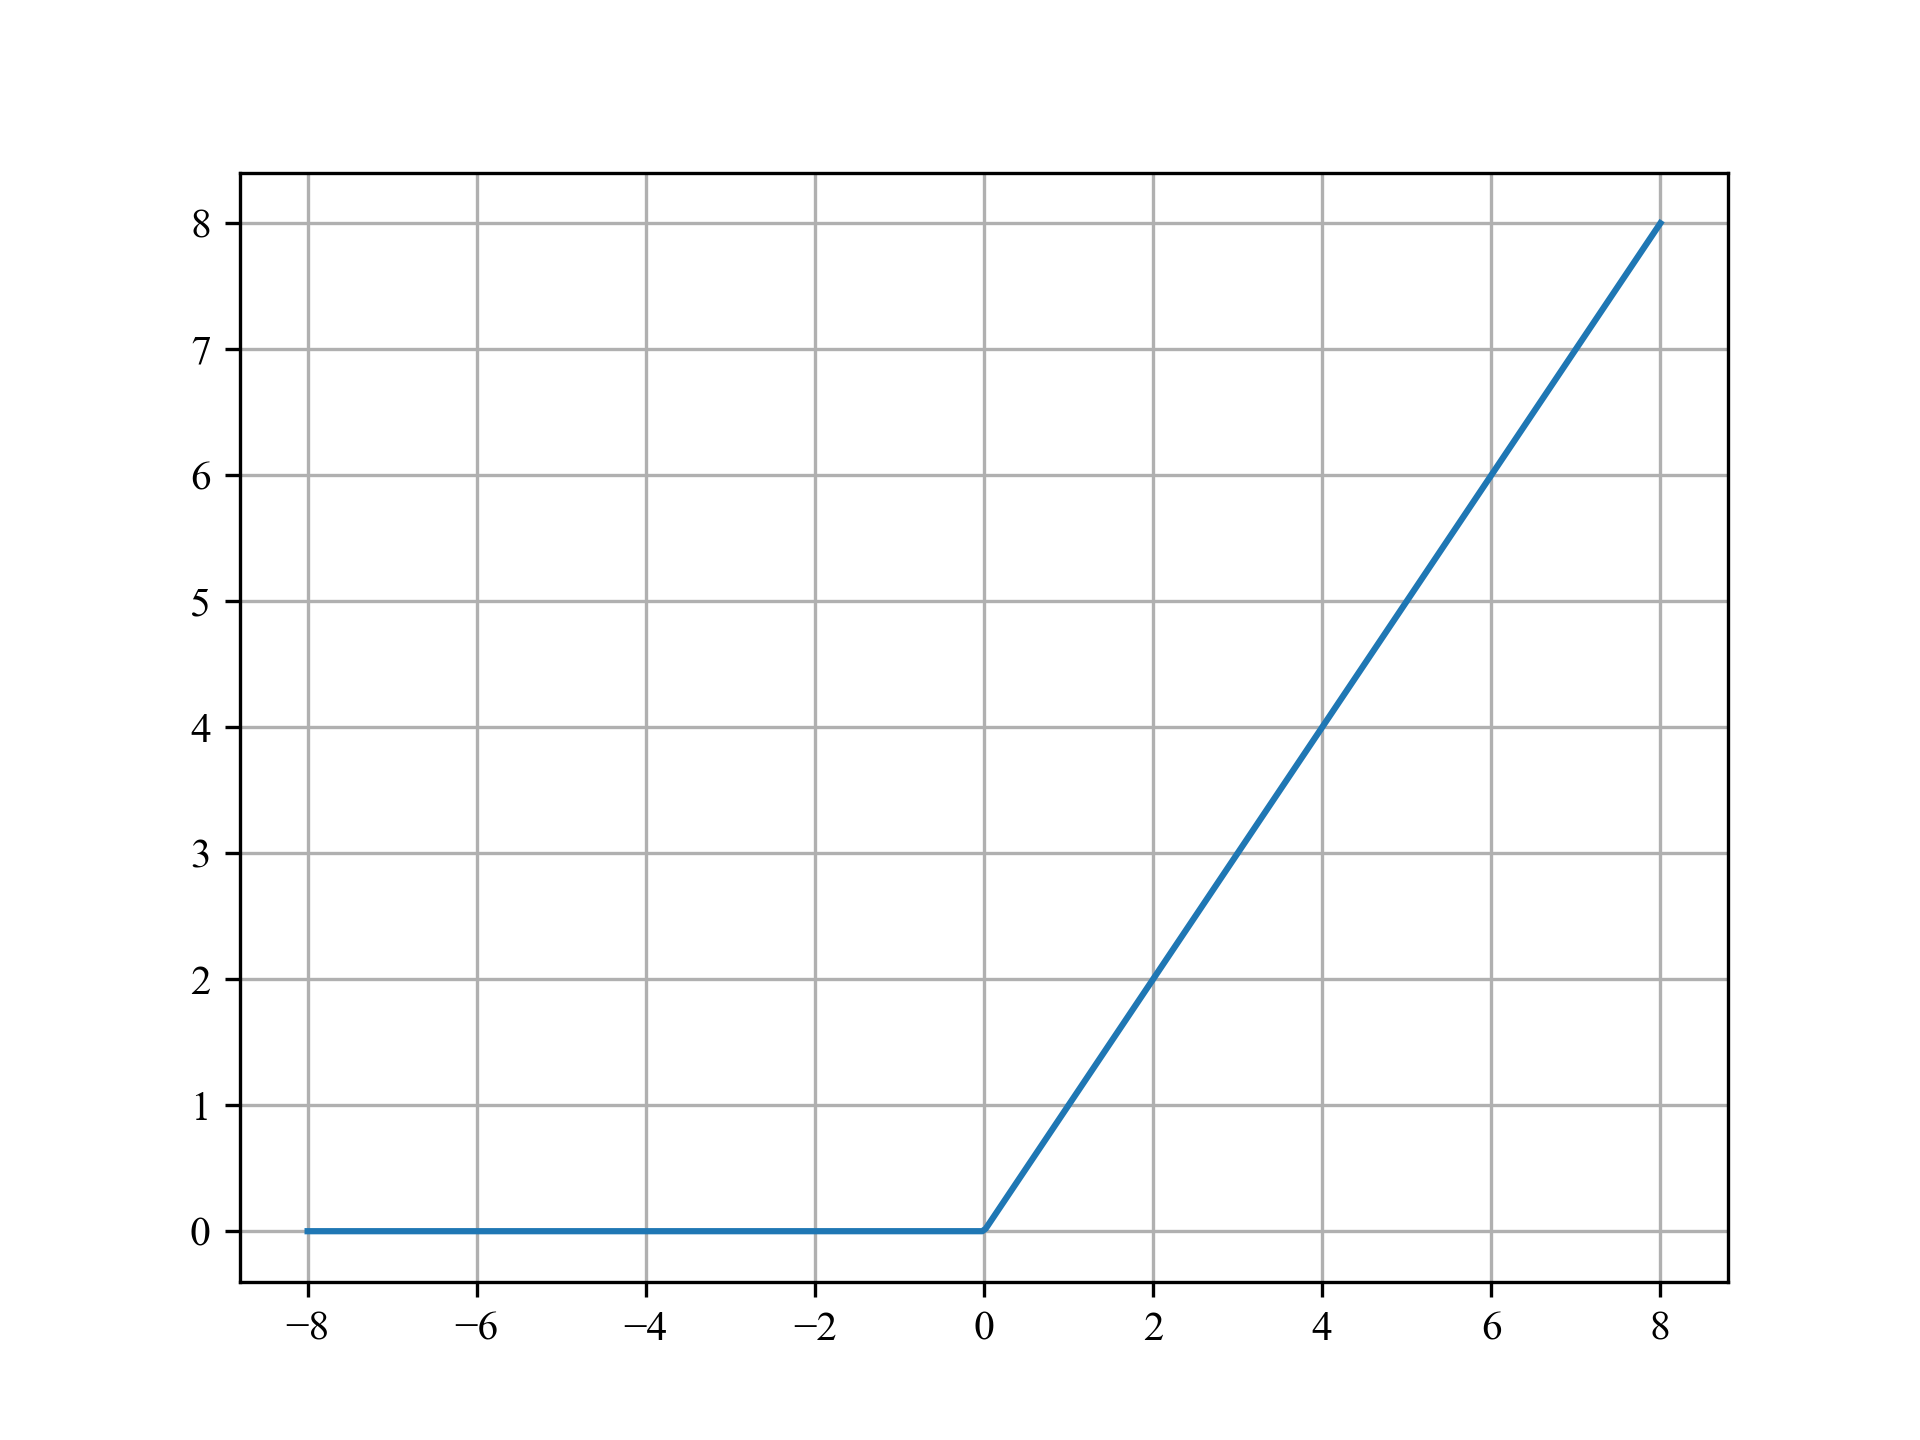
\includegraphics[width=\linewidth]{ch2/activation_function/relu.png}
    \caption{ReLU函数图像}
  \end{subfigure}
  \begin{subfigure}[t]{0.45\textwidth}
    \centering
    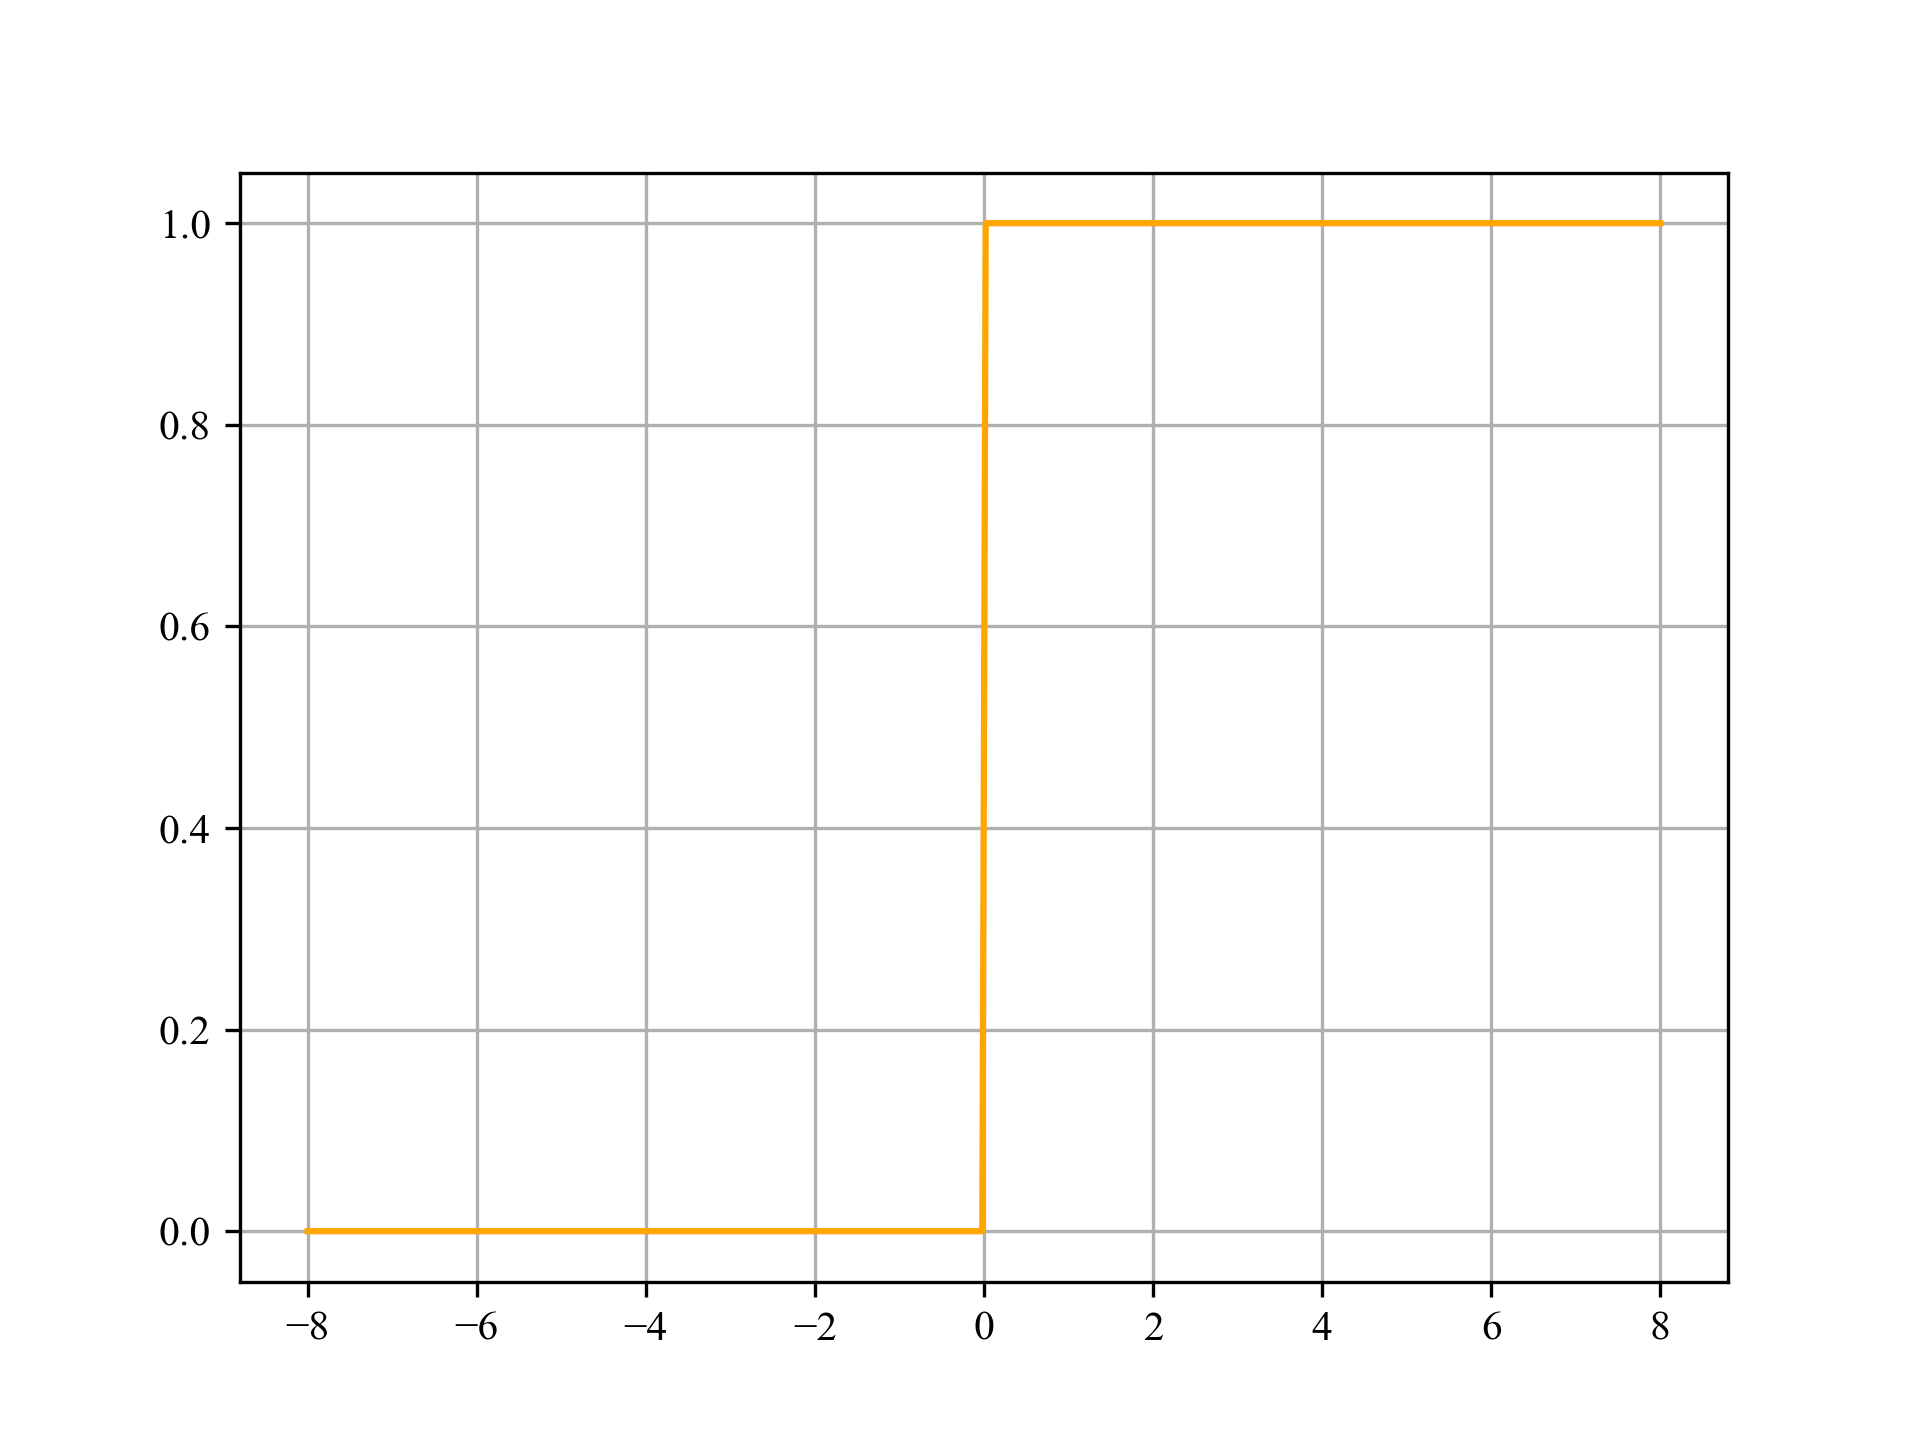
\includegraphics[width=\linewidth]{ch2/activation_function/drelu.png}
    \caption{ReLU函数导数图像}
  \end{subfigure}
  \caption{ReLU激活函数及其导数图像}
  \label{fig:relu}
\end{figure}

\subsubsection*{(3)Elu激活函数}

Elu激活函数由Clevert等人\cite{ClevertUH15}提出,旨在解决ReLU导致的神经元“死亡”问题,其计算方式如公式\eqref{eq:elu}所示:
\begin{equation}
  \begin{aligned}
  \text{ELU}(x) &= \begin{cases}
  x, & x \geq 0, \\
  \alpha \left(e^x - 1\right), & x < 0,
  \end{cases} \\
  \text{ELU}'(x) &= \begin{cases}
  1, & x \geq 0, \\
  \alpha e^x, & x < 0.
  \end{cases}
  \end{aligned}
  \label{eq:elu}
\end{equation}

Elu函数的图像如图\ref{fig:elu}所示。当输入大于0时,该函数行为类似于ReLU,其导数接近1,有助于保持梯度稳定,加快收敛速度;
当输入小于0时,Elu采用指数函数进行平滑衰减,使得激活值可以为负,有助于减少神经元“死亡”的情况。
同时,Elu函数引入了额外的超参数$\alpha$来控制负值部分的衰减程度。

\begin{figure}[H]
  \centering
  \begin{subfigure}[t]{0.45\textwidth}
    \centering
    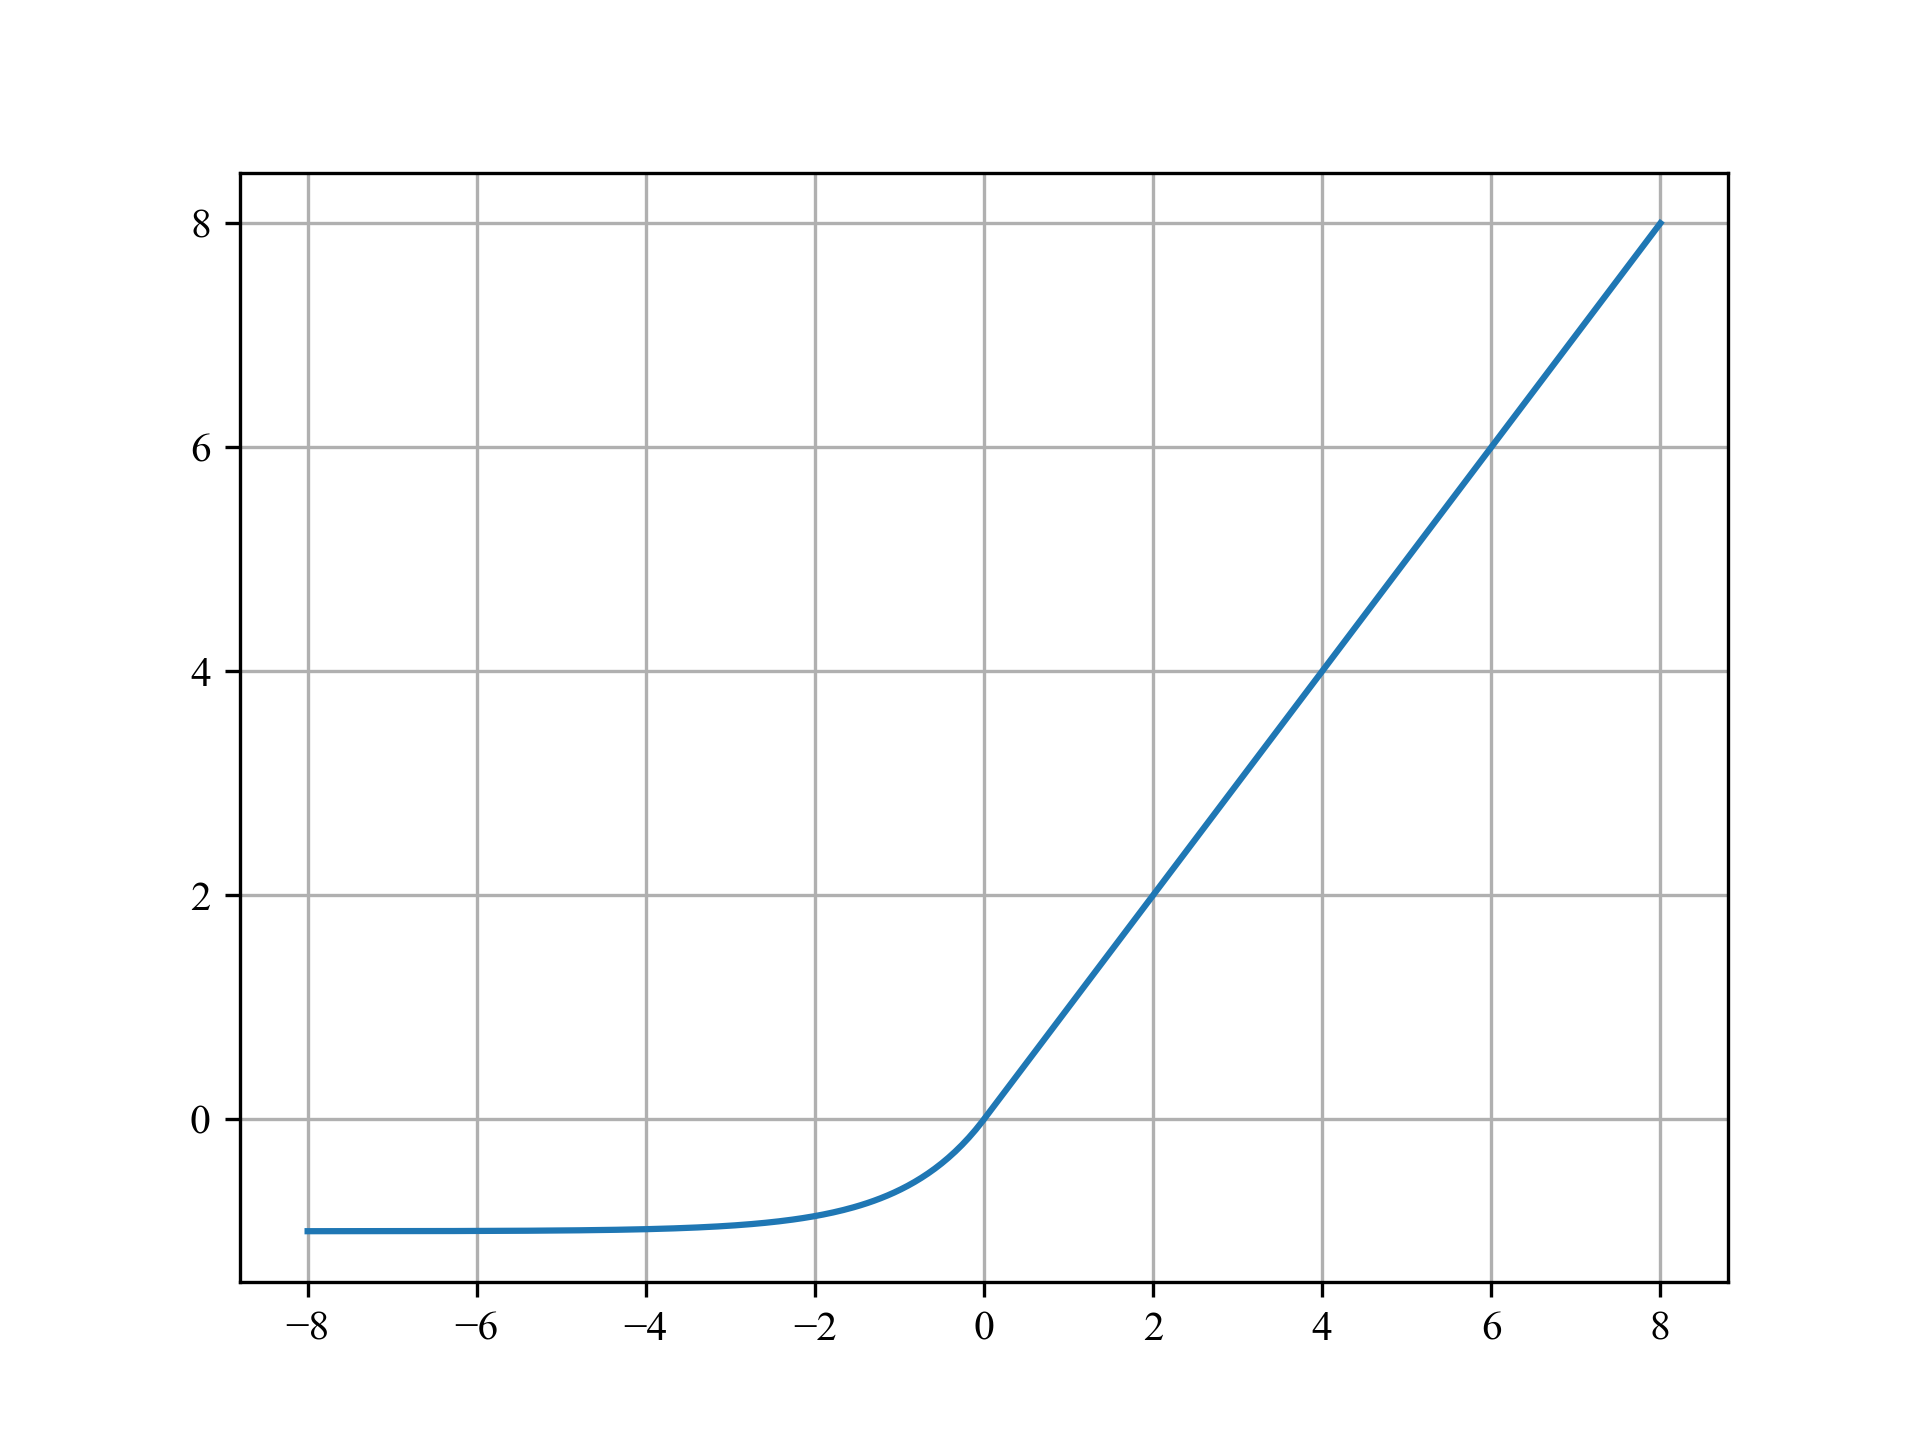
\includegraphics[width=\linewidth]{ch2/activation_function/elu.png}
    \caption{Elu函数图像}
  \end{subfigure}
  \begin{subfigure}[t]{0.45\textwidth}
    \centering
    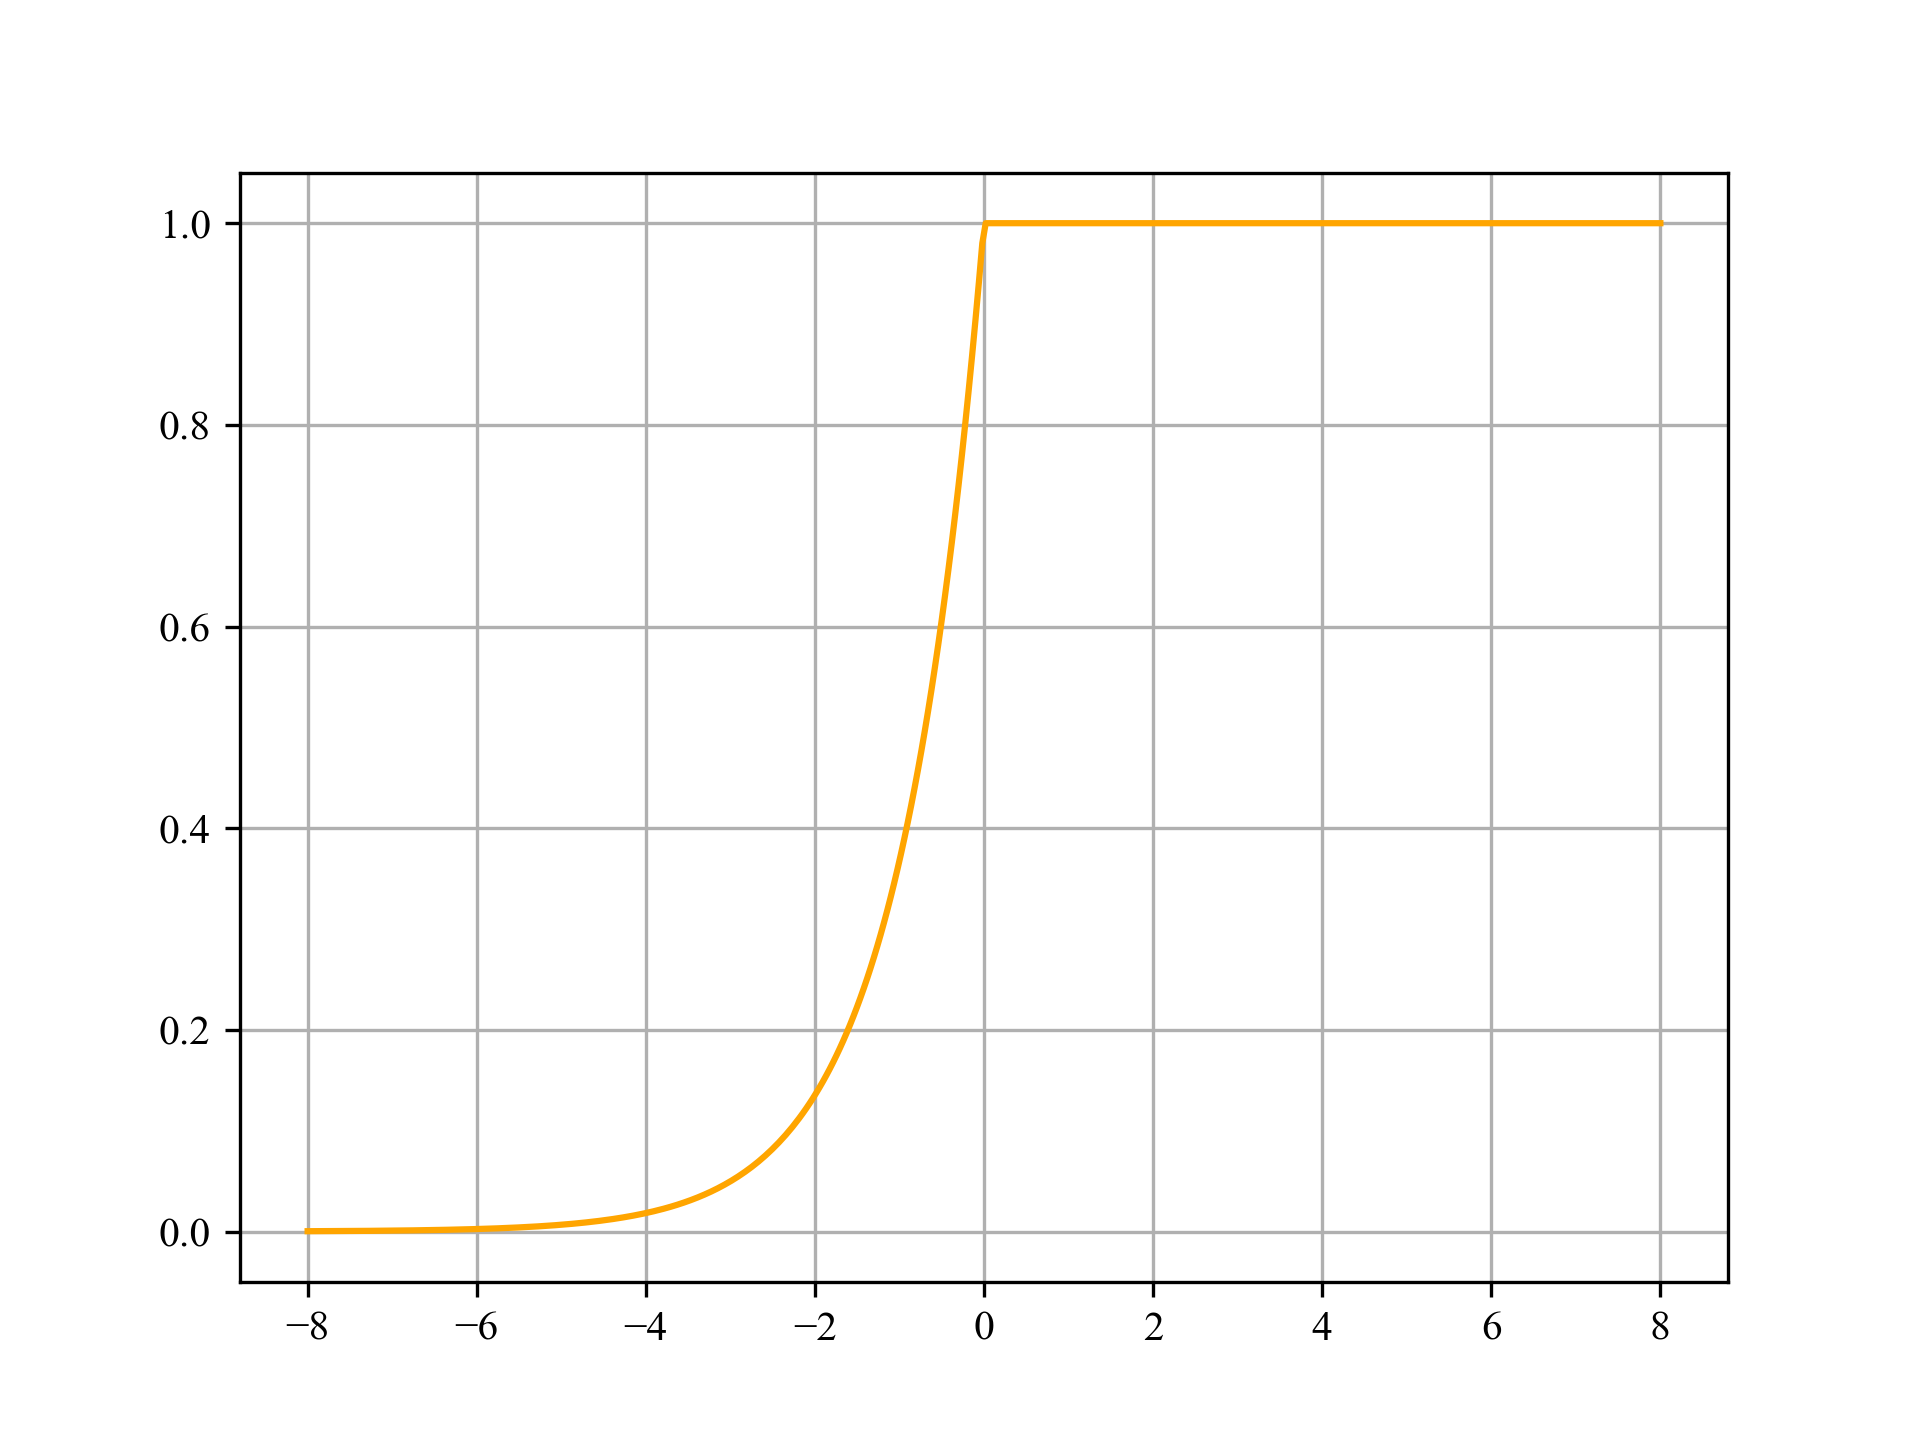
\includegraphics[width=\linewidth]{ch2/activation_function/delu.png}
    \caption{Elu函数导数图像}
  \end{subfigure}
  \caption{Elu激活函数及其导数图像}
  \label{fig:elu}
\end{figure}

\subsubsection*{(4)Sinusoid激活函数}

Sinusoid激活函数使用周期性的正弦函数,其输出范围在$[-1,1]$,由Sitzmann等人\cite{sitzmann2020implicit}
提出并应用于SIREN(Sinusoidal Representation Networks)。
\begin{equation}\label{eq:siren}
\phi_i(x_i)=\sin\Bigl(\lambda\,{\boldsymbol{W}}_i\,x_i+b_i\Bigr)
\end{equation}
其中,$\lambda$ 是可学习的频率缩放系数,决定了正弦函数的振荡速率,${\boldsymbol{W}}_i$为权重矩阵。
Sinusoid激活函数及其导数的图像如图\ref{fig:sinusoid}所示。
\begin{figure}[H]
  \centering
  \begin{subfigure}[t]{0.45\textwidth}
    \centering
    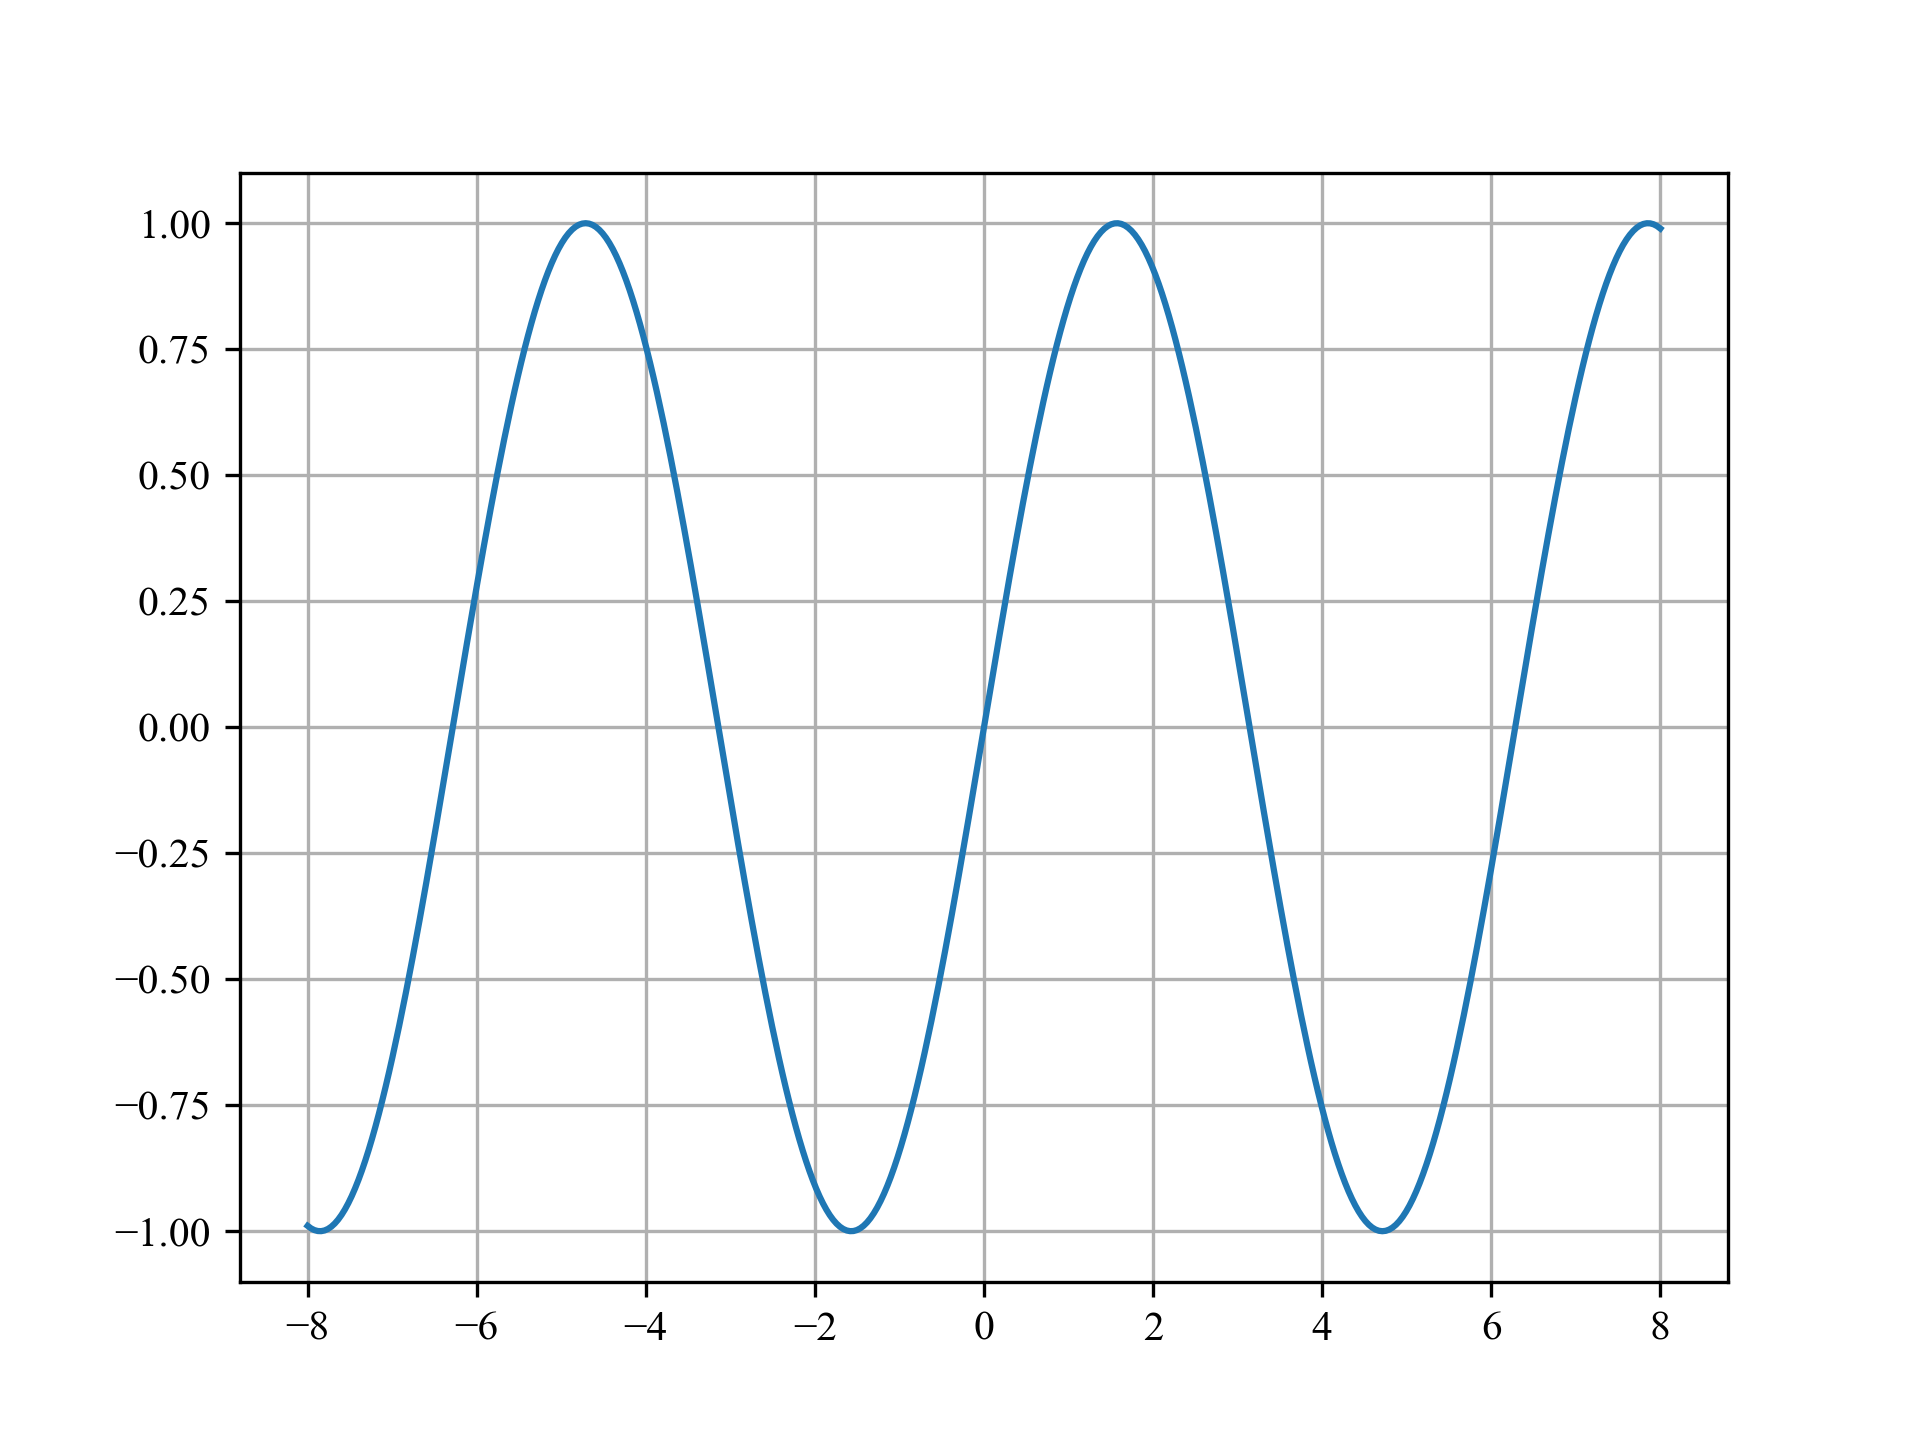
\includegraphics[width=\linewidth]{ch2/activation_function/siren.png}
    \caption{Sinuoid函数图像}
  \end{subfigure}
  \begin{subfigure}[t]{0.45\textwidth}
    \centering
    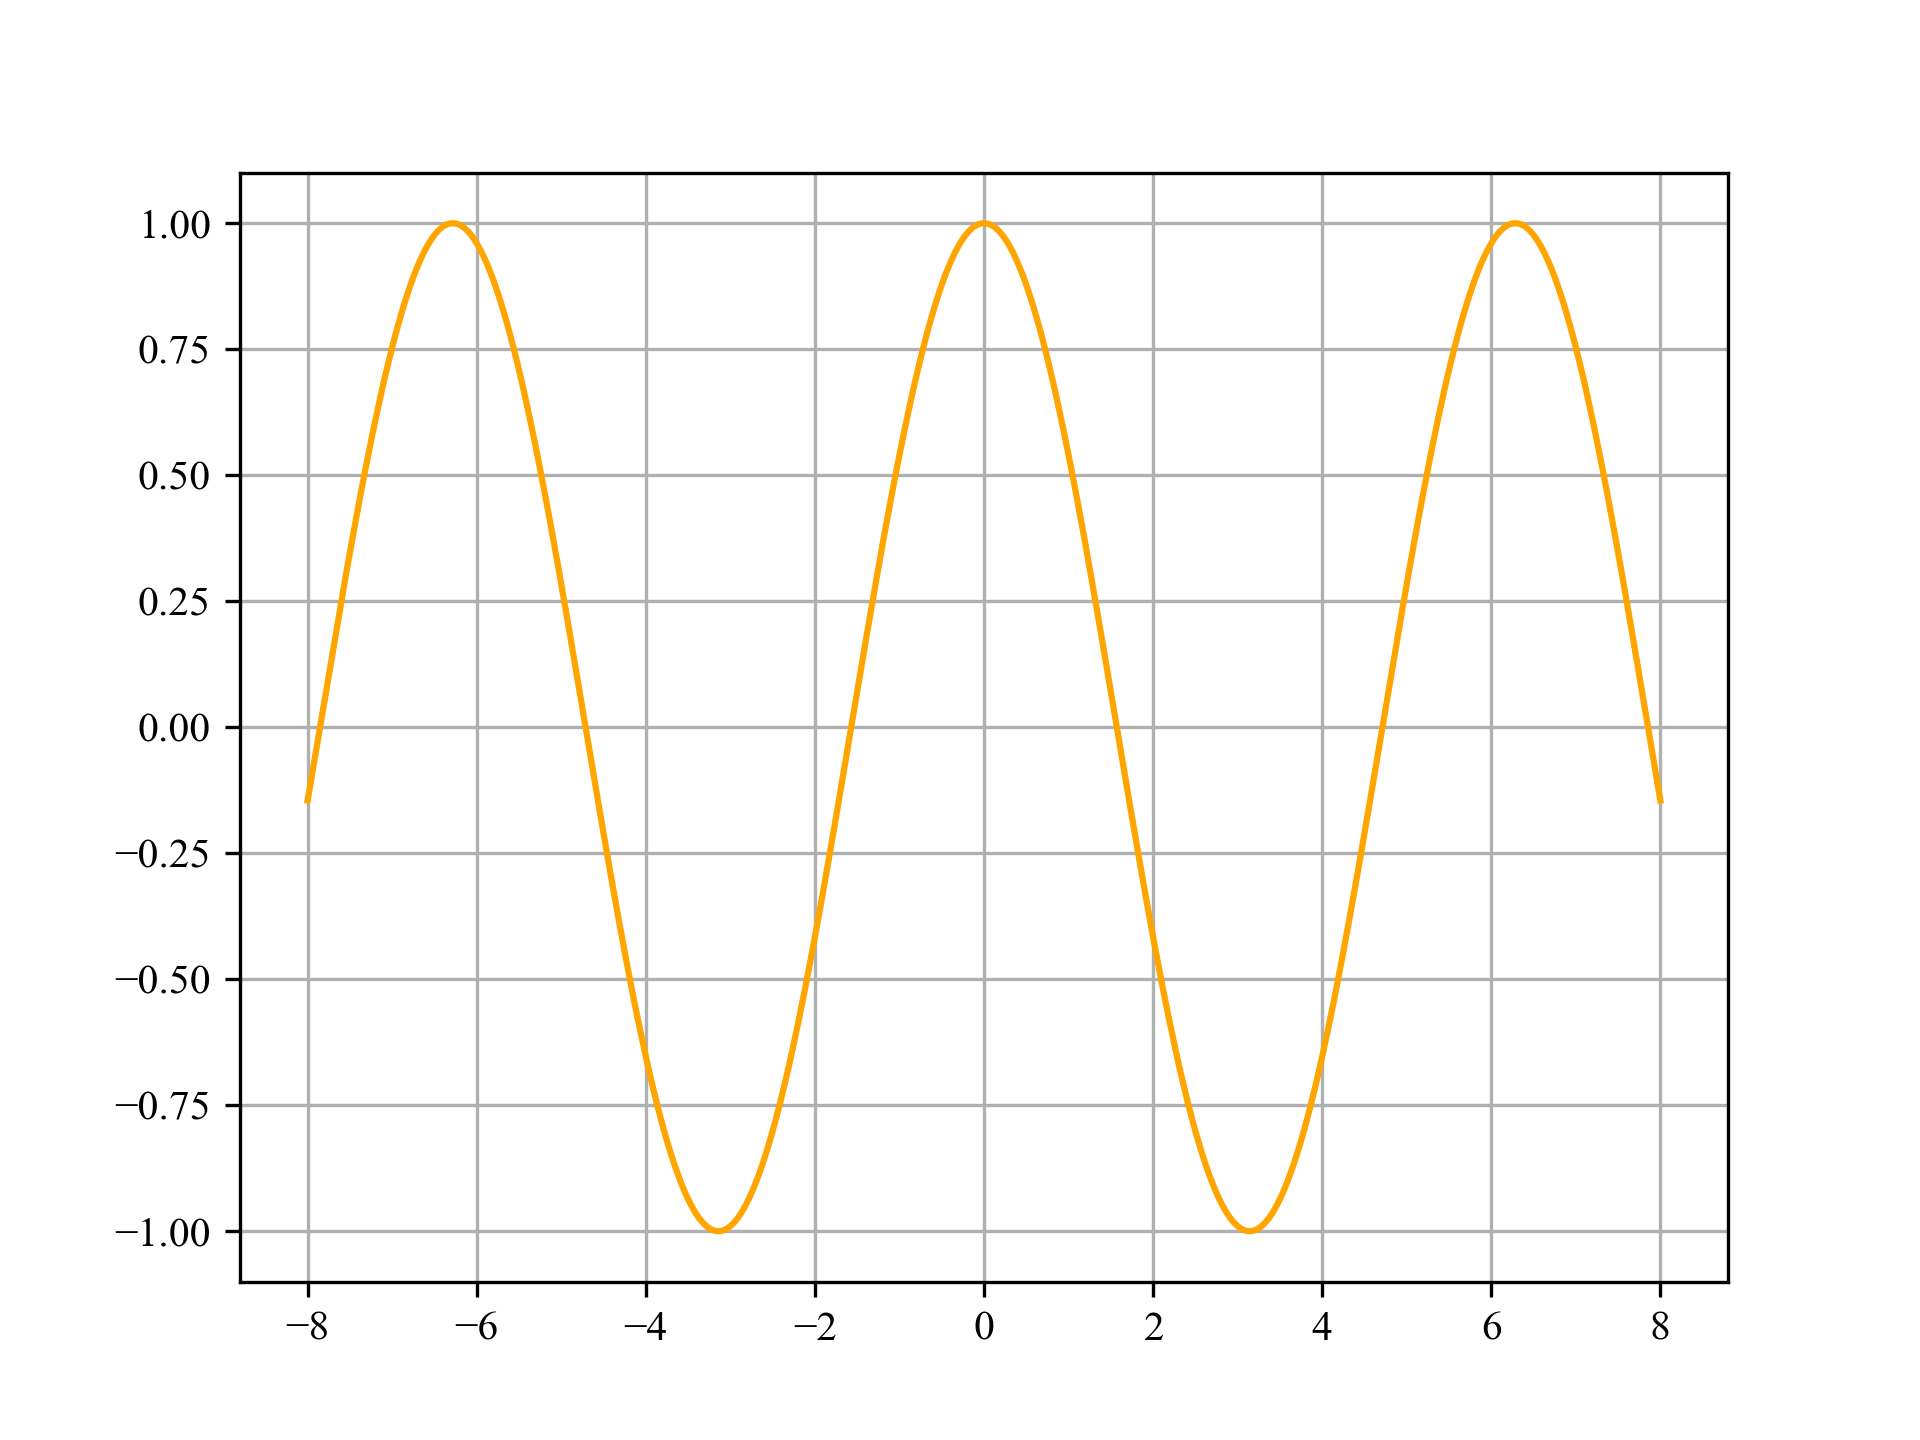
\includegraphics[width=\linewidth]{ch2/activation_function/dsiren.png}
    \caption{Sinuoid函数导数图像}
  \end{subfigure}
  \caption{Sinuoid激活函数及其导数图像}
  \label{fig:sinusoid}
\end{figure}

Sinusoid激活函数与ReLU等常见激活函数不同,由于其了使用正弦函数,因此具备独特的周期性,
能够让网络更自然地表示高频信息,权重矩阵${\boldsymbol{W}}_i$与频率系数$\lambda$则共同影响输入信号的频域分布,
使网络能够自适应地平衡低频轮廓和高频细节的建模能力,如图\ref{fig:siren_compare}所示。

\begin{figure}[htb]
  \centering
  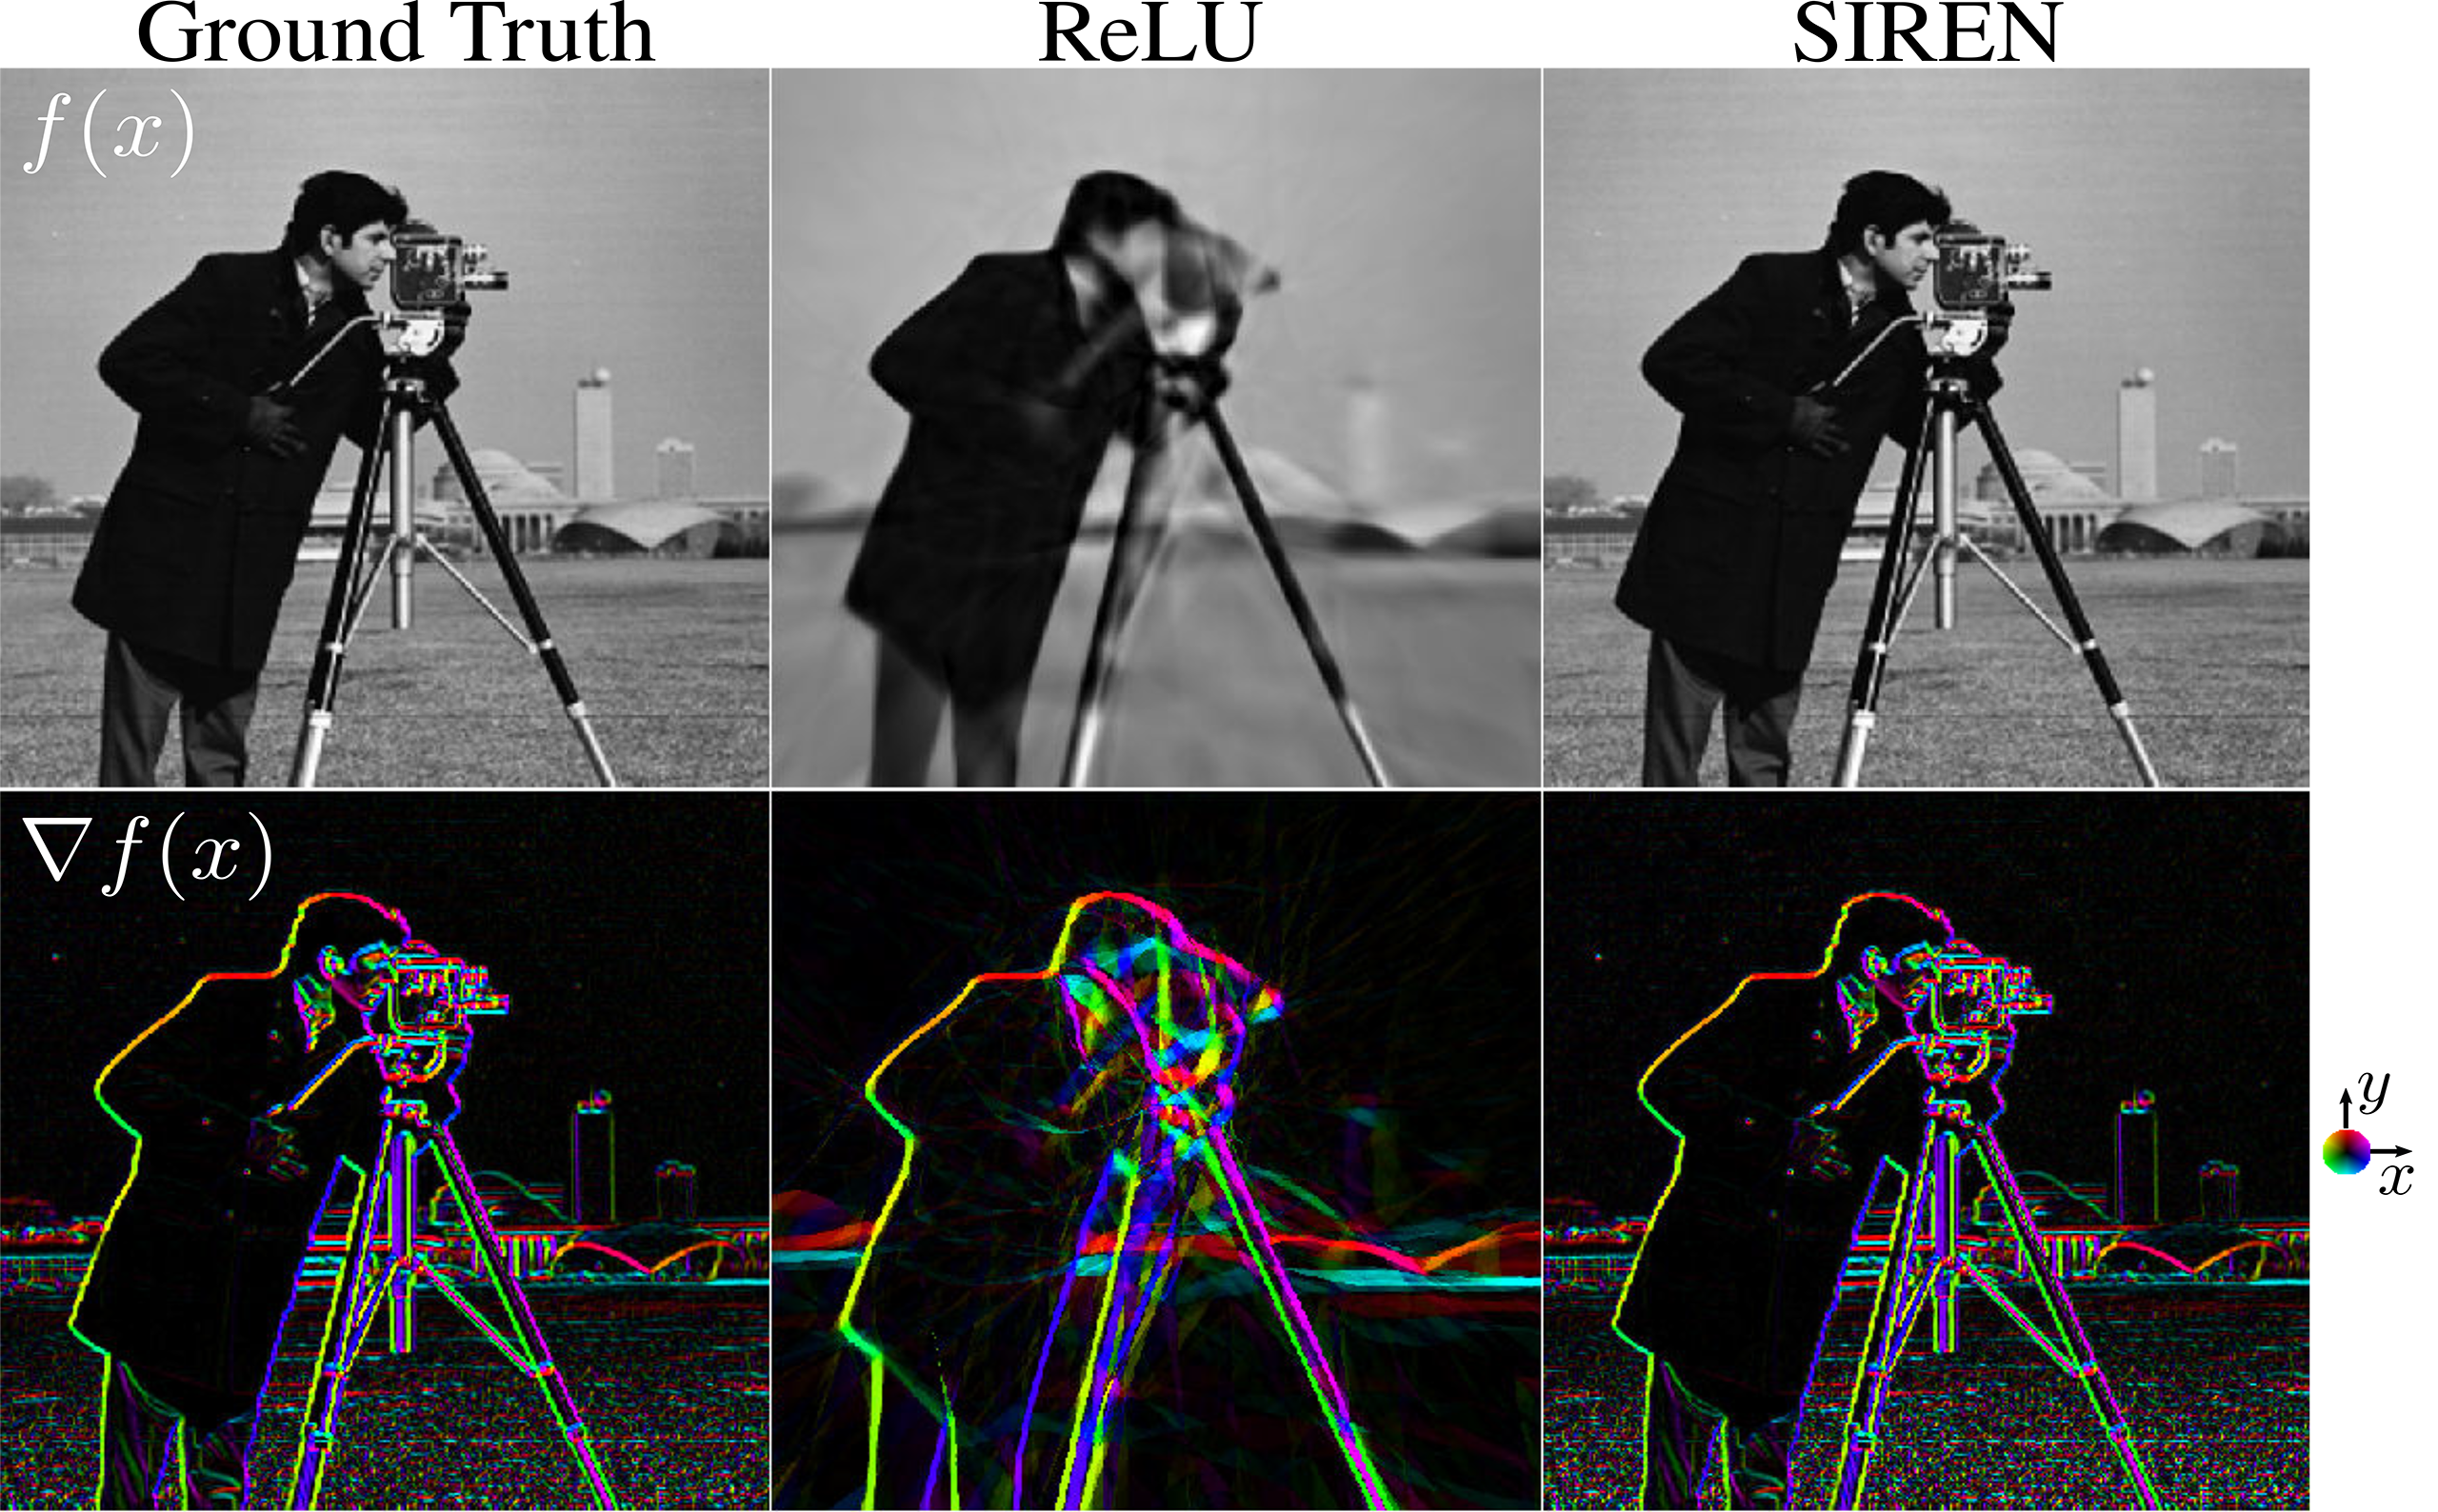
\includegraphics[width=0.7\linewidth]{ch2/Siren.png}
  \caption{激活函数对比\cite{sitzmann2020implicit}}
  \label{fig:siren_compare}
\end{figure}

\subsection{损失函数}

损失函数的作用是量化模型预测结果与真实值之间的差异。网络通过反向传播算法计算损失函数对参数的梯度,
并利用梯度下降法等优化方法更新参数,从而逐步缩小预测与真实值的差距。在训练过程中,
损失函数的值通常随着迭代下降,但过度追求较低的损失值可能导致过拟合等问题。

实际应用中,不同类型的任务需要根据不同的数据特征选择合适的损失函数。在回归问题中,
网络的输出是连续的数值,因此通常选择均方误差(Mean Squared Error,MSE)损失函数来评估预测与真实数值之间的距离。
具体定义为:
\begin{equation} 
  \mathcal{L}_{\text{MSE}}=\frac{1}{n}\sum{i=1}^{n}\left|y_i - \hat{y}_i\right|^2 
\end{equation}
其中$y_i$表示真实值,$\hat{y}_i$表示模型预测值,$n$为数据样本的数量。
均方误差直观且易于优化,广泛应用于图像重建、信号预测等任务中。

除了基本的损失函数外,在神经网络训练中经常会引入正则化项,以实现对模型参数或输出结果的额外约束。
正则化项通过添加额外的损失值来引导模型学习更加合理、平滑的结果,避免出现过拟合或不理想的局部特征。
当处理图像重建或几何优化问题时,过拟合的网络通常会导致输出结果产生大量高频伪影,
这时就可以引入平滑正则化项来引导网络的输出更加平滑。
常见的平滑正则化方法包括全变分(Total Variation,TV)正则化,其定义为:
\begin{equation} 
  \mathcal{L}_{\text{TV}}(\boldsymbol{I})=\sum_{i,j}\sqrt{\left(I_{i+1,j}-I_{i,j}\right)^2+\left(I_{i,j+1}-I_{i,j}\right)^2} 
\end{equation} 
其中$I_{i,j}$代表图像在像素位置$(i,j)$的数值。通过最小化该项,可以有效减少图像中的噪声和不规则的变化,使结果变得更加平滑。

正则化项还防止参数过多的模型出现过拟合问题,$L_2$正则化通过对网络权重施加平方范数约束,
使模型倾向于选择权重较小的解,从而有效地提高模型的泛化性能。
$L_2$正则化项可以由以下公式定义:
\begin{equation}
  \mathcal{L}_{\mathrm{L_2}}=\sum{k}\left|\omega_k\right|^2 
\end{equation} 
其中,$\omega_k$表示模型中的第$k$个参数,$\lambda$ 为控制正则化强度的权重超参数,数值越大,$L_2$正则化项的约束效果越强。

\subsection{自动编码器} \label{sec:auto_encoder}
自动编码器(Autoencoder)是深度学习中一种重要的无监督学习方法,其思想来源于生物感知系统中对信息进行压缩与重建的机制。
自动编码器通常由两个网络组成:编码器(Encoder)和解码器(Decoder)。编码器负责将输入数据压缩成一个更简单、
更紧凑的表示;解码器则根据压缩后的表示,尽可能准确地重建出原始数据。在这个过程中,
网络通过最小化输入与重建输出之间的差异来学习数据中本质的特征。

从数学角度理解,自动编码器可以视作一种降维工具:给定输入数据$x\in\mathbb{R}^D$,
编码器$\mathcal{E}$首先将其映射为低维潜空间向量$z\in\mathbb{R}^d$中;随后,
解码器$\mathcal{D}$再尝试由潜空间表示重构原始输入,即$\hat{x}=\mathcal{D}\left(\mathcal{E}\left(x\right)\right)$。
自动编码器的训练过程可通过以下优化目标实现:
\begin{equation}\label{eq:ae_loss}
\min_{\theta,\phi}E_{x\sim p_{\mathrm{dt}}}\Bigl[\bigl|x-\mathcal{D}_\phi\bigl(\mathcal{E}_\theta(x)\bigr)\bigr|^2\Bigr]
\end{equation}
其中,$\theta$和$\phi$分别表示编码器和解码器的网络参数。通过这样的优化,网络能够自动地发现数据内在的低维结构,
因此在特征提取、降维和去噪等实际问题中有广泛的应用。

对于可微渲染任务来说,自动编码器能够有效地提取特征并压缩数据。
可微渲染中的光照场景往往以高分辨率图像表示,例如一张$256\times256$大小的环境贴图可能包含数百万个像素,
直接优化这些高维数据非常困难。一方面,直接对高维数据进行优化容易陷入局部最优点;另一方面,具备真实感的光照信息必须施加额外约束,
而传统方法仅通过人工设计的正则项难以完全满足这些约束。
真实的光照场景中存在一些更简单、更规律的低维特性,
例如主光源的位置、颜色分布等,但显式地描述这些规律需要专业且精准的先验知识。
而自动编码器的“压缩重建”机制可以将复杂的光照数据被压缩至低维潜空间,使得光照表示更加紧凑且易于优化。
编码器所定义的潜空间还能捕捉光照的核心特征,使得输出结果同时满足物理约束条件。
这样,原本复杂的优化问题就转变为在一个平滑且低维的潜空间内搜索最优解,极大地提高了优化效率。

\section{传统渲染管线}
本节介绍传统渲染管线的相关基础概念,为本文针对工作流进行光照分解补充背景知识。传统渲染管线中,
数字资产通常由网格体和多张纹理贴图组成,其中,网格体表达了数字资产的几何形状,纹理贴图和各类参数表达了数字资产表面不同的光学属性。
本节将介绍数字资产的制作和渲染过程,并解释数字资产与着色模型之间存在的耦合关系。

\subsection{渲染方程}
渲染方程(Rendering Equation)是计算机图形学中描述光与物体表面交互的基础方程之一。
由Kajiya等人于1986年提出\cite{Kajiya_1986},它为物体表面的光照计算提供了一个物理上合理的模型,
广泛应用于真实感渲染和计算机图像生成中。渲染方程通过描述光从场景中的光源到达表面并反射到观察者的过程,
计算表面点的辐射亮度(Radiance)。具体计算过程如公式\eqref{eq:rendering_equation}:
\begin{equation}
  \label{eq:rendering_equation}
  L_o\left({\boldsymbol{x}},{\boldsymbol{\omega}}_o\right)=\int_{\upOmega}f_r\left({\boldsymbol{x}},{\boldsymbol{\omega}}_i,{\boldsymbol{\omega}}_o\right)\cdot L_i\left({\boldsymbol{x}},
  {\boldsymbol{\omega}}_i\right)\left({\boldsymbol{\omega}}_i\cdot\boldsymbol{n}\right)\,\mathrm{d}{\boldsymbol{\omega}}_i
\end{equation}
其中,$L_o\left({\boldsymbol{x}},{\boldsymbol{\omega}}_o\right)$表示从表面点$\boldsymbol{x}$沿观察方向${\boldsymbol{\omega}}_o$看到的辐射亮度,
$L_i\left({\boldsymbol{x}},{\boldsymbol{\omega}}_i\right)$是从入射方向${\boldsymbol{\omega}}_i$到达表面点$\boldsymbol{x}$的光源辐射亮度,
$f_r\left({\boldsymbol{x}},{\boldsymbol{\omega}}_i,{\boldsymbol{\omega}}_o\right)$是BRDF,
它决定了光线从入射方向${\boldsymbol{\omega}}_i$到反射方向${\boldsymbol{\omega}}_o$的散射方式,且依赖于表面的材质属性。
$\left({\boldsymbol{\omega}}_i\cdot\boldsymbol{n}\right)$表示入射光与表面法线$\boldsymbol{n}$的点积,代表表面与光源的接触程度,
而$\mathrm{d}{\boldsymbol{\omega}}_i$是入射光方向的微小立体角元素。

渲染方程的核心思想是通过积分所有可能的光源对表面反射的贡献,计算出最终的观察光照。
其在实际应用中能够模拟多种光照现象,包括漫反射、镜面反射、折射以及其他复杂的光学效应。
然而,尽管渲染方程具有强大的表达能力,但其高计算成本使得在实时渲染和可微渲染中难以直接应用。
因此,许多基于渲染方程的模型需要进行简化或近似,以实现高效的图像生成。

\subsection{着色模型}

着色模型(Shading Model)是基于渲染方程的简化或近似,通常用于图形学中的实时渲染。其主要目标是通过简化光的反射过程,
使得渲染计算更加高效。通过引入一定的数学公式和参数设置,着色模型能够近似真实世界中的光照现象,
从而生成具有理想真实感或艺术效果的图像。着色模型的核心是描述光线与物体表面相互作用的数学函数,
输入通常包括入射光线、视角、表面法线以及材质属性(如漫反射颜色、镜面反射强度、粗糙度等),
输出则是某一点处的最终光照颜色或亮度。常见的着色模型包括:

\subsubsection*{(1)基于物理的着色模型}

这些模型遵循物理定律,精确描述光照现象,通常依赖于BRDF。
例如,Cook-Torrance模型\cite{Cook_1981}通过微表面分布函数、几何遮蔽因子和Fresnel反射等参数,精确地模拟了金属和非金属表面的反射行为。
基于物理的着色模型能够较为准确地模拟光的反射、折射和散射过程,生成更为真实的视觉效果。

\subsubsection*{(2)经验性着色模型}

这类模型通常采用简化或经验公式来近似光照计算,
代表性的有Blinn-Phong模型和Lambertian模型。尽管它们并不完全遵循物理定律,
但通过经验参数(如光泽度、反射系数等)的调控,依然能够生成具有一定真实感的光照效果。
由于计算复杂度较低,经验性模型广泛应用于实时渲染或资源受限的场景。

\subsection{工作流} \label{sec:workflow}
工作流(Workflow)在计算机图形学中指的是一套标准化的参数与贴图生成流程,它定义了如何结合和组合各类材质参数和贴图,
以表述数字资产表面不同的光学属性。简言之,工作流决定了如何构建数字资产的表面属性,使其能够符合特定的着色模型的计算需求。
因此,选择适当的工作流对于高效且精准地表达材质的视觉效果至关重要。

工作流与着色模型之间具有紧密的耦合关系,每种工作流设计都对应着特定的着色模型,这些模型通过接收由工作流生成的参数和贴图,
进行光照计算与视觉效果渲染。不同的工作流基于不同的物理或经验性模型,表达表面特性的方式也有所不同。
本节介绍三种工作流兼具了基于物理的以及非物理的着色模型,并且仍在现代渲染引擎和项目中广泛使用。

\subsubsection*{(1)Metallic工作流}

该工作流利用金属度(Metallic)贴图区分金属与非金属区域,使用粗糙度(Roughness)描述表面的粗糙程度。
由于该工作流直接描述物体表面的金属性质,因此渲染效果更易符合预期。在该工作流的数字资产中,共使用三张纹理:
基础色(Albedo)纹理在金属材质中表示镜面反射颜色,而在非金属中表示漫反射颜色,记为$\boldsymbol{b}$;
金属度贴图区分金属与非金属区域,记为$m$;粗糙度描述表面的粗糙程度,记为$r$。

金属度工作流可以使用微表面模型的Cook-Torrance BRDF完成计算,该模型将渲染方程中的$f_r$分为漫反射项$f_d$
以及高光反射项$f_s$:
\begin{equation}\label{eq:cook-torrance}
f_r=f_s+f_d.
\end{equation}

漫反射项$f_d$表示表面上从所有方向散射的光,通常使用Lambertian反射模型表示,即光照强度与表面法线和入射光方向的夹角无关,
只与入射光的方向有关,计算过程如下:
\begin{equation}\label{eq:lambertian}
f_d=\frac{1-m}{\pi}
\end{equation}

高光反射项$f_s$表示光线在光滑表面上按镜面反射规律反射的部分,通常依赖于入射光和观察方向与表面法线之间的角度关系,
可以被表示为:
\begin{equation}\label{eq:specular}
f_s({\boldsymbol{\omega}}_o,{\boldsymbol{\omega}}_i)=\frac{D({\boldsymbol{h}};r)\cdot F({\boldsymbol{\omega}}_o,{\boldsymbol{h}};{\boldsymbol{b}},m)\cdot G({\boldsymbol{\omega}}_i,{\boldsymbol{\omega}}_o,{\boldsymbol{h}};r)}
{4\cdot({\boldsymbol{n}}\cdot{\boldsymbol{\omega}}_i)\cdot({\boldsymbol{n}}\cdot{\boldsymbol{\omega}}_o)}
\end{equation}
其中,$D$是法线分布函数(Normal Distribution Function,NDF),$F$是菲涅尔(Fresnel)反射项,$G$是几何遮蔽(Geometry)
项,$\boldsymbol{h}$是半角向量,$\boldsymbol{n}$为表面法线。针对$D$项、$F$项以及$G$项的计算,不同的研究中针对着色风格均提出了多种实现,
接下来本文将介绍主流的几种计算方法。

在大多数渲染器中,$D$项通常使用GGX\cite{walter2007microfacet}计算,使用粗糙度控制其锐利程度:
\begin{equation}\label{eq:D_ggx}
D({\boldsymbol{h}};r)=\frac{r^2}{\pi\Bigl(({\boldsymbol{n}}\cdot{\boldsymbol{h}})^2(r^4-1)+1\Bigr)^2}
\end{equation}

同时,为了在可微渲染中使用,$D$项也可以由球面高斯(Spherical Gaussians)近似计算为:
\begin{equation}\label{eq:Dsg}
D_{\rm{SG}}({\boldsymbol{n}};r)=\frac{1}{\pi r^4}\exp\Biggl(\frac{2}{r^4}\Bigl({\boldsymbol{n}}\cdot{\boldsymbol{h}}-1\Bigr)\Biggr)
\end{equation}

F项可以根据Schlick等人\cite{schlick1994inexpensive}的研究近似计算,由如下公式给出:
\begin{equation}
  \label{eq:F}
  F({\boldsymbol{\omega}}_o,{\boldsymbol{h}};{\boldsymbol{b}},m)=F_0+\bigl(1-F_0\bigr)\Bigl(1-({\boldsymbol{\omega}}_o\cdot{\boldsymbol{n}})^5\Bigr)
\end{equation}
其中,$F_0$ 项可以通过公式\eqref{eq:F_0}表示为:
\begin{equation}
  \label{eq:F_0}
  F_0=0.04(1-m)+{\boldsymbol{b}}m
\end{equation}

最后,G项可以根据Heitz等人\cite{heitz2014understanding}的研究使用Smith联合遮蔽阴影函数(Smith Joint Masking-Shadowing),计算方式如下:
\begin{equation}
  \label{eq:G}
  G({\boldsymbol{\omega}}_i,{\boldsymbol{\omega}}_o,{\boldsymbol{n}};r)=G_{\rm{GGX}}({\boldsymbol{\omega}}_i\cdot{\boldsymbol{n}})\,G_{\rm{GGX}}({\boldsymbol{\omega}}_o\cdot{\boldsymbol{n}})
\end{equation}
其中,$G_{\rm{GGX}}$ 由公式\eqref{eq:G_ggx}计算:
\begin{equation}
  \label{eq:G_ggx}
  G_{\rm{GGX}}(z)=\frac{2z}{(2-r^2)z+r^2}
\end{equation}

\subsubsection*{(2)Specular工作流}

该工作流通过镜面反射(Specular)贴图和漫反射(Diffuse)贴图直接控制材质表面的镜面反射与漫反射颜色,
通过光泽度(Glossiness)贴图控制镜面反射的强度和大小。Specular工作流与描述表面物理性质的Metallic工作流不同,
该工作流更为灵活,可以为材质单独指定不同的镜面反射率。例如蓝色的陶瓷材质对于Metallic工作流可能需要设置部分违反物
理直觉的值才能实现,但是使用Specular工作流时可以直接调整出真实的反射表现。

在计算上,Specular工作流也使用Cook-Torrance BRDF,区别在于部分计算方式不同。首先,对于上文中公式\eqref{eq:F}所述的菲涅尔项$F$,
Specular工作流替换了其中的$F_0$:
\begin{equation}\label{eq:F0_spec}
F_0={\boldsymbol{c}}_s
\end{equation}
其中,${\boldsymbol{c}}_s$代表镜面反射纹理包含的颜色。

在计算漫反射项$f_d$时不再根据金属度进行插值,而是使用菲涅尔项$F$作为插值系数:
\begin{equation}\label{eq:diffuse_spec}
f_d=\frac{1-F}{\pi}
\end{equation}
  这种计算方式使得即使Specular允许艺术家自由分配镜面反射和漫反射的表现,也保证了能量守恒,尽量避免出现物理不真实的问题。

\subsubsection*{(3)Blinn-Phong工作流}

该工作流基于Blinn-Phong经验性着色模型,通常依赖漫反射(Diffuse)、高光反射(Specular)贴图来模拟光照效果。其中高光反射参数在公式中实现了高光部分的近似计算,以光斑的形式提供近似的光滑观感,高光反射项$f_s$计算方式如下:
\begin{equation}\label{eq:specular_BlinnPhong}
f_s=\max(\boldsymbol{n}\cdot \boldsymbol{h},0)^\alpha
\end{equation}
漫反射部分使用Lambertian经验模型。总体的计算方式可以通过如下公式表示:
\begin{equation}\label{eq:diffuse_BlinnPhong}
f_d=\frac{1}{\pi}
\end{equation}

尽管该工作流并不严格遵循物理法则,且渲染效果无法与基于物理的模型相比拟,但它的计算开销较小,无需复杂的积分,适合用于对渲染效率有较高要求且对真实感要求较低的项目,非常适合于手机等移动端设备。

\section{可微渲染理论基础}
传统渲染过程将三维场景描述转换为二维图像,但在标准计算机图形学管线中,该过程通常是不可微的,
如遮挡判断与离散三角形选择的操作并不连续,导致难以获得有效的梯度信息。
这一特性限制了渲染在基于梯度优化的机器学习和计算机视觉任务中的应用。
可微渲染(Differentiable Rendering,DR)是一种将传统渲染过程与梯度优化方法相结合的新兴技术,
其核心理念是致力于实现从三维场景到二维图像的映射过程中的可微性,从而能够通过误差反向传播直接优化场景参数。
因此,这一技术在计算机视觉和三维重建等任务中具有重要价值。

可微渲染的核心目标是计算渲染图像相对于场景参数的梯度,即${\partial I}/{\partial \upPhi}$,
其中$I$是渲染图像,$\upPhi$包含几何、材质、光照和摄像机参数。由于渲染过程中的某些操作(如光栅化、可见性计算和光照建模)
通常具有离散性或复杂的非线性特性,使得计算其导数较为困难,不同的可微渲染方法针对这些挑战提出了解决方案。
接下来,本文将分别介绍可微渲染中常见的光照表示技术和几何形状表示方法。

\subsection{基于图像的照明} \label{sec:IBL}
由于可微渲染的性质,光照表示技术需要满足连续可微,并能够使用尽量少的参数对复杂光照环境进行建模。
在这一背景下,基于图像的光照(Image Based Lighting,IBL)技术成为广泛应用的选择。
在完整的渲染方程\eqref{eq:rendering_equation}中,常规离散光源被表示为$L_i(\boldsymbol{x},{\boldsymbol{\omega}}_i)$,
其在计算时需要考虑着色点的位置。而在IBL中则假设环境处于“无限远”状态,任何一处的光源所发出的光线都是平行的,
而且辐射强度在空间中是均匀的。这种假设使得在计算任意一点的入射光强度时,可以简化为计算$L_i({\boldsymbol{\omega}}_i)$,
仅需要入射光线的方向,而不依赖于具体的位置。IBL采用环境贴图存储光照数据,
相比离散的点光源,环境贴图能够以更高的分辨率还原光照场景中的细节,同时在可微渲染的优化过程中避免了不连续性对梯度的影响。
这种连续性确保了光照参数的可导性,从而能够在可微渲染中有效优化与光照相关的参数。

除此之外,Hill等人\cite{Hill_2014}引入了分裂和近似(Split-Sum Approximation),并将其应用于现代即时渲染中,以进一步降低计算量。
分裂和近似方法主要目的是将原本公式\eqref{eq:rendering_equation}中需要在半球上计算的高维积分
拆分成两个易于预计算并在运行时快速查表获得的部分以降低计算成本,
同时在视觉效果上几乎没有损失。分裂和近似的思想可以由公式\eqref{eq:int_approx}表示:
\begin{equation}
  \int f(x)g(x){\rm{d}}x\approx \int{f(x){\rm{d}}x} \int{g(x){\rm{d}}x}
  \label{eq:int_approx}
\end{equation}

公式\eqref{eq:int_approx}将两个函数乘积的积分近似为两个函数积分的乘积,
当该思想应用于渲染方程中的镜面反射项时,则镜面反射项可以通过以下形式近似计算:
\begin{equation}
  L({\boldsymbol{\omega}}_o)\approx 
  \int_{\upOmega}{f({\boldsymbol{\omega}}_i\cdot{\boldsymbol{n}}){\rm{d}}{\boldsymbol{\omega}}_i}
  \int_{\upOmega}{L_i({\boldsymbol{\omega}}_i)D({\boldsymbol{\omega}}_i,{\boldsymbol{\omega}}_o)({\boldsymbol{\omega}}_i\cdot{\boldsymbol{n}}){\rm{d}}{\boldsymbol{\omega}}_i}
  \label{eq:L_omega_o_approx}
\end{equation}
其中,第一项表示白色环境光照的镜面BSDF积分,取决于参数$\cos{\theta}={\boldsymbol{\omega}}_i\cdot{\boldsymbol{n}};$
第二项表示法线分布函数与入射光的积分,当采用环境贴图技术时,该项可以被视作按照不同的表面粗糙度对环境贴图进行过滤,
也可以通过Mipmap技术\cite{williams_1983}预先进行计算。通过IBL技术以及分裂和近似,着色时的计算量得以大幅减少,
因此这两项技术对于可微渲染任务来说不可或缺。

但是,IBL技术在实现过程中依赖的假设简化了光照建模的复杂性,将环境光表示为来自球面上的均匀方向分布,
而忽略了光源与场景之间的距离关系、遮挡关系。这种假设在许多传统渲染任务中是合理的,但在可微渲染中,
这种假设限制了IBL对光照空间分布的表达能力,尤其在涉及局部光照变化的场景中。例如,在阴影区域中,
光线受到物体遮挡后显著衰减,而IBL由于假定光照均匀分布于无限远,难以精确捕捉遮挡效应,
从而导致阴影处的光照表示不准确。此外,IBL的假设忽略了离散光源直接光的影响,无法精确建模光源位置与着色点之间的几何关系。
因此,在传统渲染中由点光源或聚光灯直接形成的高频光照效应(如强烈的高光或投影)也难以通过IBL实现。

\subsection{几何表示} \label{sec:geo_representation}
几何表示是可微渲染的关键组成部分,用于描述场景的几何形状。用于可微渲染的良好几何表示应该捕获
局部几何细节并表示具有任意拓扑的对象,同时还具有内存和计算效率,以便在交互式应用程序中进行快速推理。
根据实现原理,表示形式主要可以分为传统图形学中的显式表示和结合了深度学习和神经网络的隐式表示两类。

\subsubsection*{(1)显式表示} 

显式表示方法通过直接定义物体表面的几何元素实现对三维形状的描述,主要包括网格(Mesh)、点云(Dense Cloud)
和SDF三种典型形式。其中,网格表示通过顶点、边和面构成的多边形网格刻画物体形状,
其顶点可附加纹理坐标、法线及颜色等属性,具有直观可编辑的特点,且能高效利用图形硬件的加速能力。
然而,实际应用中不同存储格式的兼容性问题常需额外处理,且网格拓扑结构的刚性约束限制了其在重建任务中对高频细节的还原能力。
点云表示通常由激光扫描或立体视觉设备直接生成,具有采集便捷、密度可调的优势,但因缺乏显式拓扑关联,
其直接渲染效果粗糙且编辑灵活性不足,难以满足高质量实时交互需求。
相比之下,SDF通过为空间点赋予到表面的带符号距离值,既能以连续函数形式捕捉几何细节,
又可实现紧凑的数据存储,但其计算复杂度与空间分辨率的关系需通过特定算法优化。

\subsubsection*{(2)隐式表示} 

隐式表示通过参数化模型间接定义几何形状,近年来以神经隐式表示为核心的研究取得了显著进展。
该类方法利用神经网络$F(P_i^{xyz})$预测三维点$P_i^{xyz}\in\mathbb{R}^3$的几何属性,
其内存消耗与空间分辨率无关,理论上支持无限分辨率的表面重建。典型实现包括三种范式:
占据概率模型将几何描述转化为二分类问题,通过神经网络预测点$P_i^{xyz}$位于物体内部的概率以定义形状边界;
透明度建模则直接学习空间点的透明属性,既可表征半透明物体,也可近似非透明体的占据概率;
水平集方法将物体表面定义为隐式函数$F(P_i^{xyz})=0$的解集,通过距离函数的符号区分内外空间,
在复杂几何重建中兼具精度与计算效率优势。尽管神经隐式表示存在训练耗时、采样效率低等挑战,
但其参数化特性与拓扑无关性为高精度复杂几何建模提供了突破性解决方案,
尤其在细节还原和动态拓扑适应方面展现出独特潜力。

\subsubsection*{(3)混合表示} 

现有的隐式神经表示方法难以将生成结果直接用于下游编辑等任务,而传统的显式网格体在重建效果上有所折损,
而Shen等人\cite{shen2021deep}提出了深度行进四面体(Deep Marching Tetrahedra,DMTet),
该方法结合了SDF与网格体表示的优点,并且计算过程可微,适合用于可微渲染\cite{Laine2020ModularPF}
以及几何形状生成\cite{gao2022get3d,Liu2023One2345AS}等任务中。

DMTet使用离散的SDF表示每个顶点相对于原位置的偏移量,通过可微行进四面体层
(Differentiable Marching Tetrahedra Layer,MT)将SDF转换为三角形网格,
使得该技术能够基于SDF进行优化,并直接转换为网格体。由于这种转换能够在网络优化期间进行,避免了
传统隐式表示在管线后额外转换为网格表示时引入误差的情况。同时,DMTet也解决了直接使用网格体进行优化时,
网格体拓扑相对固定、无法表示细微高频细节的情况。

DMTet的优化过程如下,当给定一个四面体网格(Tetrahedral Grid),对于网格中的每个顶点${\boldsymbol{v}}$,
DMTet学习对应的SDF值$s$和变形向量$\upDelta\boldsymbol{v}$,随后根据学习到的SDF值生成三角形面,
构成网格体。

DMTet从SDF生成三角形面的计算方式如图\ref{fig:dmtet_calc}所示,其中,标量$s$表示SDF值,
顶点${\boldsymbol{v}}_i$的位置${\boldsymbol{v}}_i^\prime$根据$s_i$的偏移进行更新,
两个相邻顶点${\boldsymbol{v}}_i$和${\boldsymbol{v}}_j$之间的顶点${\boldsymbol{v}}_{ij}$通过线性插值进行计算。

\begin{figure}[htbp]
  \centering
  \begin{tikzpicture}[
    dot/.style args={#1}{circle, fill=#1, inner sep=0pt, minimum size=3pt},
    dashedge/.style={dashed, thick}
  ]
  \definecolor{ag}{rgb}{0.0, 0.5, 0.0}
  \definecolor{ar}{rgb}{0.8, 0.0, 0.0}
% 第一个三角形(左)
\coordinate (A) at (0,0);
\coordinate (B) at (4,0);
\coordinate (C) at (2,3.464);

\draw[dashedge,line width=1.5pt,color=gray!40] (A) -- (B) -- (C) -- cycle;

% 顶点圆点(红/绿)
\filldraw[white] (A) circle(0.15);
\filldraw[white] (B) circle(0.15);
\filldraw[white] (C) circle(0.15);

\draw[color=ag!90,dashedge,line width=1.5pt] (A) circle (0.15);
\draw[color=ag!90,dashedge,line width=1.5pt] (B) circle (0.15);
\draw[color=ar!80,dashedge,line width=1.5pt] (C) circle (0.15);

% 第二个三角形(右)
\coordinate (A') at (0.5,-0.25);
\coordinate (B') at (4.3,0.7);
\coordinate (C') at (1.3,3.1);

\draw[dashedge,line width=1.5pt,color=black!90] (A') -- (B') -- (C') -- cycle;

\filldraw[white] (A') circle(0.15);
\filldraw[white] (B') circle(0.15);
\filldraw[white] (C') circle(0.15);

\filldraw[ag,fill opacity=0.8] (A') circle(0.15);
\filldraw[ag,fill opacity=0.8] (B') circle(0.15);
\filldraw[ar,fill opacity=0.8] (C') circle(0.15);

% 在两条边上添加额外圆点
\coordinate (M1) at ($(B')!.6!(C')$);
\coordinate (M2) at ($(A')!.4!(C')$);

% 连接额外圆点的实线
\draw[line width=1.5pt,color=black!90] (M1) -- (M2);

\filldraw[white] (M1) circle(0.15);
\filldraw[white] (M2) circle(0.15);
\filldraw[gray,fill opacity=0.8] (M1) circle(0.15);
\filldraw[gray,fill opacity=0.8] (M2) circle(0.15);

% 右侧公式标注
\node[anchor=west] at (4.5,0.4) {
  $\begin{aligned}
    {\boldsymbol{v}}'_i=&{\boldsymbol{v}}_i+\upDelta{\boldsymbol{v}}_i \\
    s_i & >  0
  \end{aligned}$
};

\node[anchor=west] at (3.0,2.2) {
  $\displaystyle {\boldsymbol{v}}'_{ij}=\frac{{\boldsymbol{v}}_i\cdot s_j - {\boldsymbol{v}}_j\cdot s_i}{{s_j-s_i}}$
};

\node[anchor=west] at (-0.2,2.9) {
  $s_j < 0$
};
\end{tikzpicture}
\caption{DMTet计算三角形面的过程}
\label{fig:dmtet_calc}
\end{figure}

\newpage
\section{NeRF理论基础}
本节介绍NeRF的基本理论知识和框架。NeRF通过融合辐射场建模与可微分体积渲染,
实现了从多视角二维图像建立三维场景隐式表示的能力。本章节将详细介绍神经辐射场的基本理论框架、关键技术要点。

\subsection{NeRF的基本定义}
NeRF作为计算机视觉领域的一项前沿进展,延续了基于坐标的多层感知机以空间坐标为输入的基本架构,
但其建模对象从单一几何属性升级为辐射场函数。NeRF的基本原理是通过深度学习将三维空间中的点映射到其对应的颜色和密度,
本身的功能可以用公式\eqref{eq:nerf_mapping}定义:
\begin{equation}
  F_{\upTheta}:({\boldsymbol{x}},{\boldsymbol{d}})\rightarrow({\boldsymbol{c}},\sigma)
  \label{eq:nerf_mapping}
\end{equation}
其中,$\mathrm{x}\in\mathbb{R}^3$表示三维场景内的坐标,$\mathrm{d}\in\mathbb{S}^\boldsymbol{2}$
表示观察方向的方位角和极角,$\mathrm{c}\in\mathbb{R}^3$表示场景在$\mathrm{x}$点、于观察方向$\mathrm{d}$
进行观察时的RGB颜色,$\sigma$表示场景在$\mathrm{x}$点的密度,物理意义该点为是否存在物质或光学吸收现象,
函数$F_{\upTheta}$由一个或多个MLP完成实现。NeRF的总体框架如图\ref{fig:nerf_pipe}所示。
\begin{figure}[htbp]
  \centering
  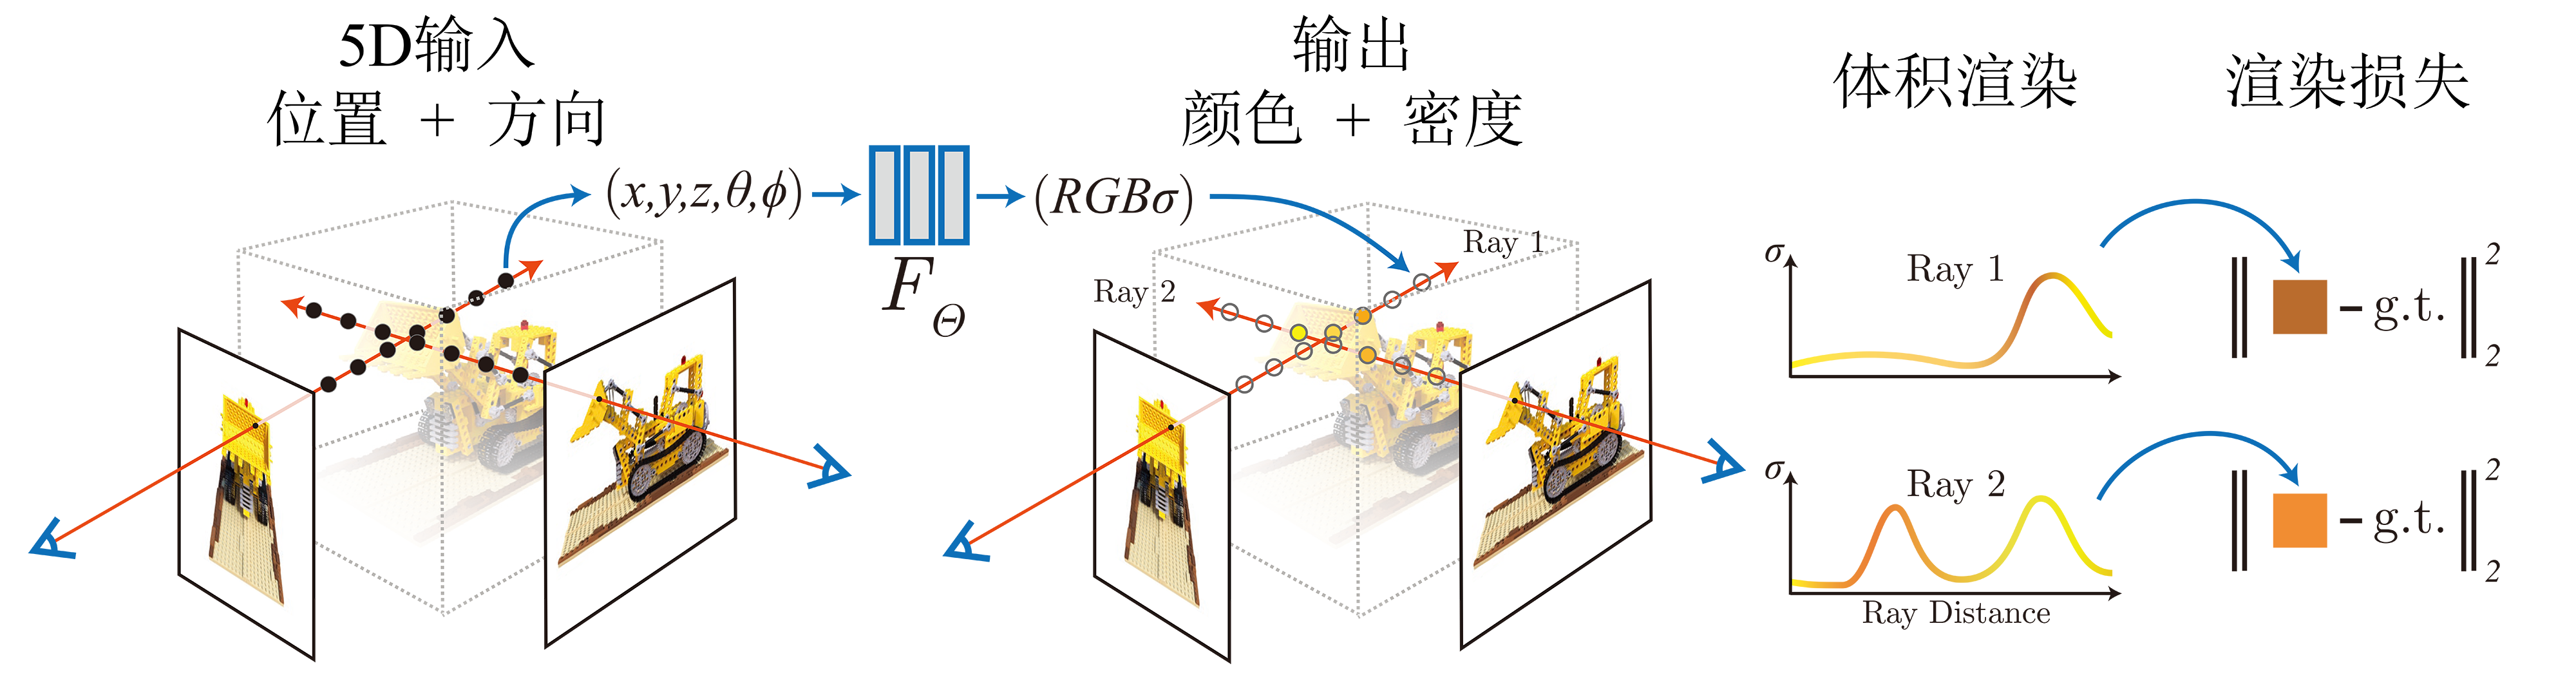
\includegraphics[width=1.0\textwidth]{ch1/NeRFPipe_lowres.png}
  \caption{NeRF训练和渲染过程\cite{Mildenhall_2020}}
  \label{fig:nerf_pipe}
\end{figure}

NeRF的基础结构使用了前文介绍的基于坐标的多层感知机,并利用公式\eqref{eq:fourier_encoding}表示的傅里叶变换对
输入坐标$\boldsymbol x$进行了位置编码,显著提升了NeRF对高频几何细节的重建能力。

\subsection{NeRF的体积渲染}

本节介绍如何通过NeRF通过观察方向$\boldsymbol d$计算输出像素颜色$\boldsymbol c$。
这一过程的核心是通过体积渲染(Volume Rendering)方法来合成二维图像。
体积渲染将沿着每条射线对函数$F_{\upTheta}$输出的颜色和密度进行积分,计算射线的最终输出颜色$\boldsymbol c$,该过程可以由以下公式表示:
\begin{equation}\label{eq:volume_rendering}
C=\int_{t_n}^{t_f}T(t)\,\sigma(r(t))\,{\boldsymbol c}(r(t),{\boldsymbol d})\,\mathrm{d}t
\end{equation}
其中,$t_f$和$t_n$分别代表沿着射线方向积分的起始和结束时刻。对沿方向$\boldsymbol{d}$发射的光线$r$,
其$t$时刻所到达的点为$r(t)$。$\boldsymbol{c}$是三维空间中给定点$r(t)$在观察方向为$\boldsymbol{d}$时的颜色,
$\sigma$是点$r(t)$的密度,颜色$\boldsymbol c$和密度$\sigma$由函数$F_{\upTheta}$计算。$T(t)$是从相机到$t$时刻位置的透射率,
$T(t)$的定义如下所示:
\begin{equation}\label{eq:transmittance}
T(t)=\exp\Biggl(-\int_{t_n}^{t}\sigma(r(s))\,\mathrm{d}s\Biggr)
\end{equation}

$T\left(t\right)$是体密度函数,$r\left(s\right)$是光线路径上的点。神经辐射场接受空间中点的坐标$\left(x,y,z\right)$
以及射线的出发点和方向作为输入,然后输出在该点的颜色和密度,对射线上所有采样点的颜色和密度进行积分求和,
即可得到最终成像图像对应像素的颜色和密度。

\subsection{衡量指标}

本节介绍与NeRF技术相关的一系列研究领域中,用来评估管线渲染质量以及几何重建质量的常用衡量指标。

\subsubsection*{(1)峰值信噪比} 

峰值信噪比(Peak Signal-to-noise Ratio,PSNR)是一种基于均方误差(Mean-square Error,MSE)
来计算图像之间绝对差异的方法,其计算过程简单直观,能够有效反映图像重构过程中细节信息的丢失或噪声引入问题,
PSNR的高低直接揭示了光照输出图像与原始真实图像在整体灰度层面上的恢复效果。
因此,PSNR能够为本文方法的有效性提供了直观且定量的参考依据,其计算公式为:
\begin{equation}\label{eq:PSNR}
\mathrm{PSNR}=10\cdot\log_{10}\frac{\mathrm{MAX}_\mathrm{I}^2}{\mathrm{MSE}}
\end{equation}
其中,$\mathrm{MAX}_\mathrm{I}$表示图像中可能的最大像素值,而$\mathrm{MSE}$定义为:
\begin{equation}\label{eq:MSE}
\mathrm{MSE}=\frac{1}{mn}\cdot\sum_{i=1}^{m}\sum_{j=1}^{n}\Bigl[I(i,j)-K(i,j)\Bigr]^2
\end{equation}
这里$I$和$K$分别代表原始图像和重建图像,$m\times n$为图像尺寸。

\subsubsection*{(2)结构相似性指标} 

尽管PSNR在衡量像素级误差方面具有优势,但它无法全面捕捉图像中人眼感知的结构信息。
为此,本文同时采用了结构相似性指标(Structural Similarity,SSIM)来补充评估。
SSIM从亮度、对比度和局部结构三个方面对图像相似性进行综合考量,更符合人眼对图像质量的直观感受,
从而为评估重渲染图像的视觉一致性提供了更为全面和精细的判断,其基本公式可以分解为三个部分:
\begin{equation}\label{eq:SSIM}
\mathrm{SSIM}(x,y)=\Bigl[l(x,y)\Bigr]^\alpha\cdot\Bigl[c(x,y)\Bigr]^\beta\cdot\Bigl[s(x,y)\Bigr]^\gamma
\end{equation}
其中,$l(x,y)$、$c(x,y)$、$s(x,y)$分别用于衡量亮度、颜色和对比度差异,各部分的权重$\alpha$、$\beta$、$\gamma$通常被设定为1,使得整体SSIM值介于0到1之间,其中1代表两幅图像完全相同。

\subsubsection*{(3)学习感知图像块相似度} 

学习感知图像块相似度(Learned Perceptual Image Patch Similarity,LPIPS)是一种基于深度学习的图像质量评价指标,
旨在从人类视觉感知的角度衡量两幅图像之间的差异。与PSNR和SSIM等传统方法不同,LPIPS通过预训练的卷积神经网络
(Convolutional Neural Network,CNN)提取图像的高层语义特征,并在特征空间中计算图像块的感知相似性。
其核心思想是模仿人类视觉系统对图像内容的理解能力,能够更准确地捕捉图像在纹理、边缘和语义结构上的细微差异,
从而更符合主观视觉质量的评判标准。

LPIPS的计算过程可概括为以下步骤:首先,将待比较的原始图像和重建图像分别输入预训练的CNN
(如VGG \cite{journals/corr/SimonyanZ14a}或AlexNet \cite{NIPS2012_c399862d}),
提取多层特征图;随后,对每层特征图进行归一化处理,并计算对应特征通道之间的L2距离;最后,
通过加权平均各层距离得到最终的相似度得分。其数学表达式为:
\begin{equation}\label{eq:lpips}
  \mathrm{LPIPS}(x,y)=
  \sum_{l}\frac{1}{H_{l}\times W_{l}}
  \sum_{h,w} \Bigl \Vert w_{l} \odot \Bigl(F_{l}^{(x)}(h,w)-F_{l}^{(y)}(h,w) \Bigr) \Bigr \Vert_{2}^{2}
\end{equation}
其中,$x$和$y$为输入图像对,$F_{l}^{(x)}$和$F_{l}^{(y)}$分别表示第$l$层网络提取的特征图,
$H_{l}\times W_{l}$为特征图尺寸,$w_{l}$为对应层的可学习权重向量,$\odot$表示逐通道相乘。LPIPS值越低,
表明两幅图像在感知上越相似。本文引入LPIPS指标,旨在弥补传统方法在复杂纹理、
语义一致性等高层视觉特征评估上的不足。相较于PSNR和SSIM,LPIPS能够更敏感地反映人眼对图像细节失真、
内容扭曲的感知差异,从而为光照重建模型的视觉保真度提供更深入的量化分析依据。

\subsubsection*{(4)倒角距离}

倒角距离(Chamfer Distance,CD)是一种用于衡量三维点云或几何表面之间空间相似性的度量方法,
可以用来衡量NeRF及光照分解管线对几何形状的重建效果。其核心思想是通过计算两组点集中每个点到另一组点集的最近邻距离之和,
量化二者在几何结构上的匹配程度。CD值越低,表明两个点集的几何结构越接近,即重建效果越好。
CD的数学表达式为:
\begin{equation}\label{eq:CD}
\mathrm{CD}(P,Q)= \sum_{p \in P} \min_{q \in Q} \|p - q\|^2 + \sum_{q \in Q} \min_{p \in P} \|p - q\|^2
\end{equation}
其中,\(P\) 和 \(Q\) 分别表示两个待比较的点集(例如分别由网格体采样得到的点云),\(\|\cdot\|\) 表示欧氏距离。
在实际应用中,为了准确反映网格体的形状信息,通常会对网格表面进行均匀采样,生成点云后再计算Chamfer Distance。
同时,实验中报告的数值单位常以 \(10^{-3}\) 为标准,例如一个数值为5的CD指标实际上表示\(5 \times 10^{-3}\)的距离。
这样,CD不仅可以作为模型训练过程中的损失函数,也能作为评估生成结果与真实形状相似度的直观量化指标。

\section{本章小结}
在本章节中,本文全面回顾了本文研究所依赖的关键技术基础,包含了深度学习、传统渲染管线、可微渲染理论以及NeRF的相关知识。

深度学习是本文工作的重要基础,其使得对数字资产的解耦成为可能。本文首先介绍了深度学习中的基础网络结构——基于坐标的MLP。
随后介绍了相关的激活函数、损失函数等概念。对于MLP在三维几何隐式建模中的应用,傅里叶位置编码和正弦激活函数有效解决了
传统激活函数在高频细节捕捉上的不足。最后,本文讨论了自动编码器在光照参数压缩与重构中的作用。

由于本文工作旨在无缝对接传统渲染器,因此本章梳理了渲染方程及常见着色模型的基本原理,
并介绍了数字资产制作流程与其对应的着色模型。

接着,本章阐述了可微渲染的概念,指出传统渲染过程中因离散操作而导致的不可微性问题,
进一步总结了基于不同几何表示的可微渲染方法及其各自的优缺点。

最后,本章着重对NeRF技术进行了介绍。NeRF是一项基于坐标MLP和可微体积渲染的方法,能够从多视角二维图像重建三维场景的结构与外观。
这项技术拓展了三维场景重建与新视角合成任务的可能性,同时为本文研究提供了重要的技术与理论支撑。
